%****************************************************************************%
%* DIET User's Manual main file                                             *%
%*                                                                          *%
%*  Author(s):                                                              *%
%*    - Philippe COMBES (Philippe.Combes@ens-lyon.fr)                       *%
%*                                                                          *%
%* $LICENSE$                                                                *%
%****************************************************************************%
%* $Id$
%* $Log$
%* Revision 1.6  2004/01/15 23:59:31  ecaron
%* Add corrections from Holly Dail
%*
%* Revision 1.5  2003/12/15 00:13:53  ecaron
%* New structure for the first sheet
%*
%* Revision 1.4  2003/12/12 14:42:44  pkchouha
%*  define \diet_version in UserManual.tex to be 1.0
%*
%* Revision 1.3  2003/12/12 12:36:17  ecaron
%* Change call to diet_initialize()
%* Correct some bug
%*
%* Revision 1.2  2003/09/17 14:41:28  pcombes
%* Split the .tex according to its chapters.
%*
%* Revision 1.1  2003/09/09 12:38:20  pcombes
%* Reorganization of doc: UM becomes UsersManual.
%*
%* Revision 1.9  2003/06/16 17:40:33  pcombes
%* Date
%*
%* Revision 1.8  2003/05/23 09:23:35  pcombes
%* Add suggestions from Jean-Yves. Thanks !
%*
%* Revision 1.7  2003/05/15 14:17:58  pcombes
%* UM 0.7
%*
%* Revision 1.4  2003/01/22 17:34:53  pcombes
%* User Manual, v. 0.6.4
%*
%* Revision 1.3  2003/01/21 12:17:02  pcombes
%* Update UM to API 0.6.3, and "hide" data structures.
%*
%* Revision 1.2  2003/01/13 12:09:00  pcombes
%* UM: client part complete for users's day ...
%*
%* Revision 1.1.1.1  2002/12/13 17:06:34  pcombes
%* User's Manual - architecture
%****************************************************************************%

\documentclass[12pt,a4paper]{book}
\makeatletter
\makeatother
\usepackage{fancyheadings}
\usepackage[headings]{fullpage}
%\usepackage[french]{babel}
%\usepackage[latin1]{inputenc}
%\usepackage{multicol}
\usepackage{verbatim}
\usepackage{url}
\usepackage{subfigure}

\usepackage{graphicx}
\graphicspath{{./fig}}

\newsavebox{\logobox}
\sbox{\logobox}{
\includegraphics[scale=0.3]{fig/logo_DIET.ps}}
\newcommand{\logo}{\usebox{\logobox}}



%%%%
\renewcommand{\title}{DIET User's Manual}
%%%%

\pagestyle{fancyplain}
\lhead[\fancyplain{\title}{\title}]
      {\fancyplain{\title}{\title}}
\chead{}
\rhead[\fancyplain{\logo}{\logo}]{\fancyplain{\logo}{\logo}}

\lfoot[\fancyplain{INRIA}{INRIA}]{\fancyplain{INRIA}{INRIA}}
\cfoot[\fancyplain{}{}]{\fancyplain{}{}}
\rfoot[\fancyplain{Page~\thepage}{Page~\thepage}]
      {\fancyplain{Page~\thepage}{Page~\thepage}}


\newcommand{\ptop}{\textit{Peer-to-Peer}}
\newcommand{\red}{\textit{Red}}
\newcommand{\sci}{Scilab}
\newcommand{\scip}{Scilab$_{//}$}
\newcommand{\scalapack}{ScaLAPACK}
\newcommand{\sed}{\textit{SeD}}
\newcommand{\thread}{\textit{thread}}
\newcommand{\threads}{\textit{threads}}
\newcommand{\nsl}{NetSolve}
\newcommand{\fixme}[1]{\fbox{\textsl{{\bf #1}}}}
\newcommand{\dietversion}{1.0}

%%%%
% Document beginning
%%%%

\begin{document}



%%%%
% First sheet
%%%%

\thispagestyle{empty}
\vspace*{3cm}
\vspace*{3cm}

\begin{center}
\includegraphics[scale=.5]{fig/LOGO_DIET.ps}\\[2ex]
\textbf{\Huge USER'S MANUAL\\[2ex]}
\end{center}

\vfill


\noindent
\small{
\begin{tabular}{ll}
  \textbf{VERSION}  & 1.0\\
  \textbf{DATE}     & December 2003\\
  \textbf{PROJECT MANAGER}  & Fr\'ed\'eric \textsc{Desprez}.\\
  \textbf{EDITORIAL STAFF}  & Eddy \textsc{Caron} and Philippe ~\textsc{Combes}.\\
  \textbf{AUTHORS STAFF}    & 
\begin{minipage}[t]{12cm}
  Eddy \textsc{Caron}, Pushpinder Kaur \textsc{Chouhan}, Philippe ~\textsc{Combes},
  Sylvain \textsc{Dahan}, Bruno \textsc{Delfabro}, Georg \textsc{Hoesch}, Christophe \textsc{Pera}, Cyrille \textsc{Pontvieux}, Jean-Yves \textsc{L'Excellent} and Antoine \textsc{Vernois}.
\end{minipage} \\
  \textbf{Copyright}& INRIA
\end{tabular}\\
}

\newpage
\thispagestyle{empty}
\ 

%%%%
% End of first sheet
%%%%


\newpage
\tableofcontents


%
% Introduction
%
\newpage
\addcontentsline{toc}{chapter}{Introduction}
\chapter*{Introduction}


DIET stands for Distributed Interactive Engineering Toolbox. It is a
toolbox for easily developing Application Service Provider systems,
based on the Client/Agent/Server scheme. In DIET, user's requests are
served via RPC.

The RPC paradigm~\cite{CM00,MNS+00} is a good candidate for building
to build Problem Solving Environments (PSE) for numerical applications
on the Grid~\cite{HR00}. Several tools following this approach exist,
such as \nsl~\cite{nug}, NINF~\cite{NSS99}, NEOS~\cite{FMM00}, or
RCS~\cite{AGM97}. They are most commonly referred to as Network
Enabled Server (NES) environments~\cite{MNS+00}. Such environments
usually have five different components: \emph{Clients} that submit
problems they have to solve to \emph{Servers}, a \emph{Database} that
contains information about software and hardware resources, a
\emph{Scheduler} that chooses an appropriate server depending on the
problem sent and the information contained in the database, and
finally \emph{Monitors} that acquire information about the status of
the computational resources.

But \nsl\ and NINF have a centralized scheduler which can become a
bottleneck when many clients try to access several servers.  Moreover
as networks are highly hierarchical, the location of this unique
scheduler has a great impact on the performance of the overall
platform.

DIET is based on the five component types described above, but a
hierarchy of schedulers (agents) are used to address the scalability
problems seen in \nsl\ and NINF. Clients always submit their to one of
a particular agent (their Master Agent or MA). Below the MA is a
hierarchy of agents (Local Agents or LA) which share the workload for
scheduling jobs.

%
% A DIET platform
%
\newpage
%****************************************************************************%
%* DIET User's Manual description chapter file                              *%
%*                                                                          *%
%*  Author(s):                                                              *%
%*    - Philippe COMBES (Philippe.Combes@ens-lyon.fr)                       *%
%*                                                                          *%
%* $LICENSE$                                                                *%
%****************************************************************************%
%* $Id$
%* $Log$
%* Revision 1.25  2009/09/07 16:07:47  bdepardo
%* Added CCS mode.
%* A few corrections:
%* - DIET -> \diet
%* - SeD -> \sed
%*
%* Revision 1.24  2008/07/17 21:54:32  ecaron
%* Update scale for figures
%*
%* Revision 1.23  2008/07/17 21:31:46  ecaron
%* To be compliant to latextohtml (use scale instead of resizebox)
%*
%* Revision 1.22  2008/07/15 23:11:44  ecaron
%* Typo
%*
%* Revision 1.21  2008/07/02 12:56:28  gcharrie
%* cosmetics and figures
%*
%* Revision 1.20  2008/06/10 16:59:56  ycaniou
%* Typos
%* Use the "${DIET_DOC_SOURCE_DIR}/../src/.." non portable to get path to .c to
%*   be included in the doc. Should be ok if the doc is not removed from the DIET
%*   project
%* Batch chapter � priori completed
%*
%* Revision 1.19  2008/06/09 08:14:33  ycaniou
%* Correction, typos and begin of // and batch chapter
%*
%* Revision 1.18  2008/04/07 22:25:38  ecaron
%* Updated files to pdflatex compilation
%*
%* Revision 1.17  2006/12/02 15:47:22  ycaniou
%* Re. minus 2 URLs web access et problem descriptions.
%*
%* Revision 1.16  2006/12/02 12:01:18  ycaniou
%* Some modifications: lecture termin�e pour cette partie
%*
%* Revision 1.15  2006/09/11 11:15:00  ycaniou
%* - Up to date documentation for parallel/batch submission
%* - Corrected wrong references
%*
%* Revision 1.14  2006/05/12 12:12:32  sdahan
%* Add some documentation about multi-MA
%*
%* Bug fix:
%*  - segfault when the neighbours configuration line was empty
%*  - deadlock when a MA create a link on itself
%*
%* Revision 1.13  2006/02/17 00:22:01  ecaron
%* Ready to release 2.1.0
%*
%* Revision 1.12  2006/01/25 16:52:55  pfrauenk
%* CoRI : renaming of the chapter performance prediction with fast
%* 	to performance prediction, add of the CoRI Usersmanual,
%* 	changes in the plugin scheduler
%*
%* Revision 1.11  2005/06/27 19:26:52  hdail
%* - Moved introduction to FAST to description section with intro to multi-MA and
%*   gave both chapter references.
%* - Changed version number to 2.0.
%* - Moved info on compiling FAST itself to fast section from install section.
%*   install section still explains how to configure DIET with FAST.
%*
%* Revision 1.10  2005/06/24 14:27:07  hdail
%* Correcting english problems & updating descriptions that are no longer true.
%*
%* Revision 1.9  2005/06/14 08:05:40  ecaron
%* FAST decribe as an example
%*
%* Revision 1.8  2005/06/01 07:28:43  alsu
%* errant letter removed!
%*
%* Revision 1.7  2005/06/01 07:21:35  alsu
%* fixing a figure labeling problem
%*
%* Revision 1.6  2005/05/29 13:51:22  ycaniou
%* Moved the section concerning FAST from description to a new chapter about FAST
%* and performances prediction.
%* Moved the section about convertors in the FAST chapter.
%* Modified the small introduction in chapter 1.
%* The rest of the changes are purely in the format of .tex files.
%*
%* Revision 1.5  2004/10/25 08:59:56  sdahan
%* add the multi-MA documentation
%****************************************************************************%

\chapter{A DIET platform}\label{ch:description}

\diet is built upon \emph{Server Daemons}. The process of scheduling
the requests is distributed amongst a hierarchy of \emph{Local Agents}
and \emph{Master Agents}. The scheduler can use resource availability
information collected from three different tools: from
NWS~\cite{WSH99} sensors which are placed on every node of the
hierarchy, from the application-centric performance prediction tool
\textsc{FAST} \cite{Qui02}, which relies on NWS information, or from
CoRI Easy, which is based on simple system calls and some basic
performance tests (see
Chapter~\ref{chapter:performance}). Figure~\ref{fig:platform} shows
the hierarchical organization of \diet.

\begin{figure}[htb]
 \begin{center}
  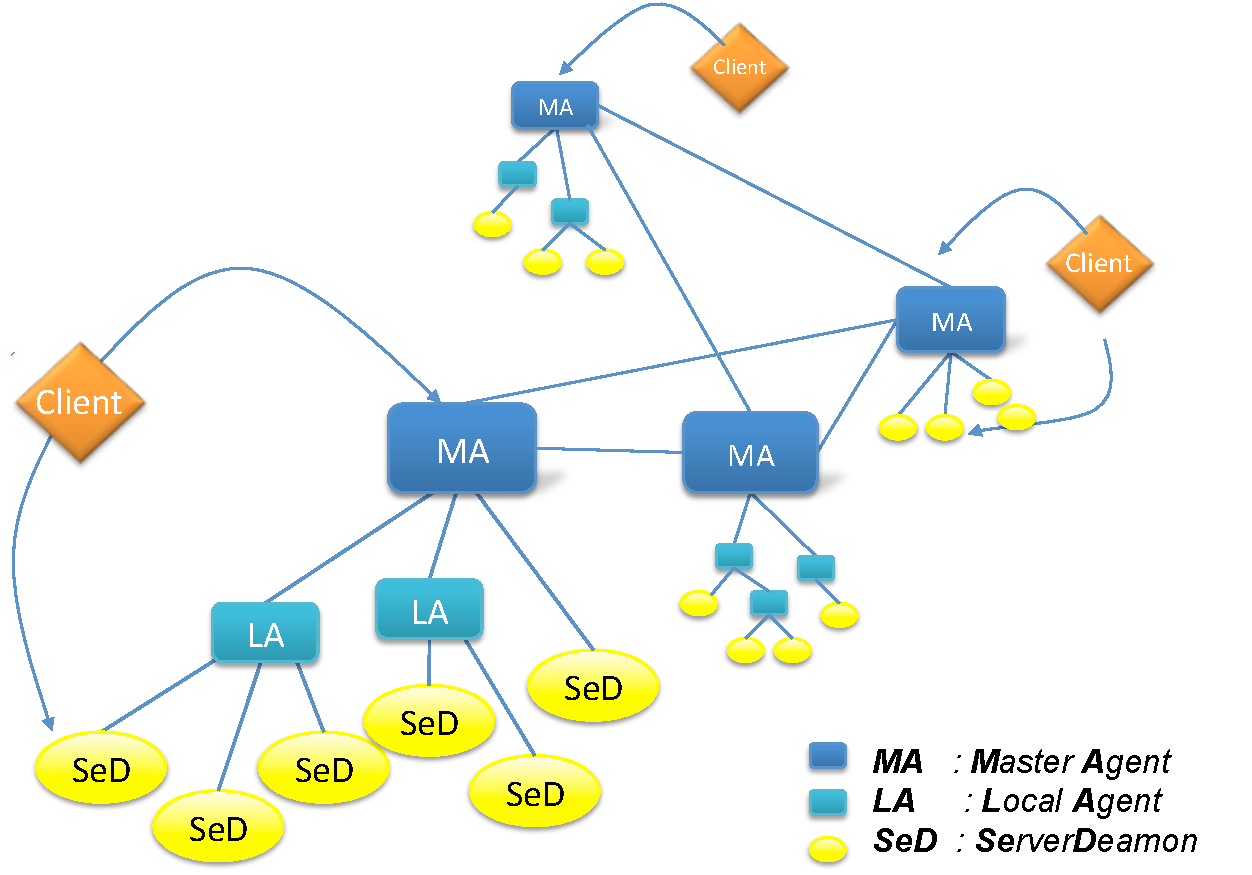
\includegraphics[scale=.7]{fig/global_platform}
  \caption{\label{fig:platform} A hierarchy of \diet agents}
 \end{center}
\end{figure}

%====[ \textsc{Diet} components ]=======================================================
\section{DIET components}
\label{sec:components}

The different components of our software architecture are the following:

\begin{description}
%....[ Client ]................................................................
\item \textbf{Client}\\ A client is an application which uses \diet to
  solve problems.  Many types of clients are able to connect to
  \textsc{Diet}, from a web page, a \pse such as Matlab or \sci, or
  from a compiled program.
%....[ Master Agent (MA) ].....................................................
\item \textbf{Master Agent (MA)}\\ An MA receives computation requests
  from clients. These requests refer to some \diet problems listed on
  a reference web page. Then the MA collects computation abilities
  from the servers and chooses the best one. The reference of the
  chosen server is returned to the client. A client can be connected
  to an MA by a specific name server or a web page which stores the
  various MA locations.

%....[ Local Agent (LA) ]......................................................
\item \textbf{Local Agent (LA)}\\ An LA transmits requests and
  information between MAs and servers.  The information stored on an
  LA is the list of services available in the subtree rooted at the
  LA; for each service, LAs store a list of children (agents or
  servers) that can be contacted to find the service. Depending on the
  underlying network topology, a hierarchy of LAs may be deployed
  between an MA and the servers. Of course, the function of an LA is
  to do a partial scheduling on its subtree, which reduces the
  workload at the MA.

%....[ Server Daemon (SeD) ]...................................................
\item \textbf{Server Daemon (\sed)}\\ A \sed encapsulates a
  computational server. For instance it can be located on the entry
  point of a parallel computer. The information stored on a \sed is a
  list of the data available locally ({\it i.e.}, on the server), the
  list of problems that can be solved on it, and performance-related
  information such as the amount of available memory or the number of
  resources available. When it registers, a \sed declares the problems
  it can solve to its parent LA or MA.  A \sed can give perfomance and
  hardware information by using the module CoRI or performance
  predictions for some types of problems by using the module FAST.
  Both modules are described in Chapter~\ref{chapter:performance}.

\end{description}

%====[ CORBA ]=================================================================
\section{Communications layer}
\label{sec:CORBA}

NES environments can be implemented using a classic socket
communication layer.  Several problems to this approach have been
pointed out such as the lack of portability or limits on the number of
sockets that can be opened concurrently.  Our aim is to implement and
deploy a distributed NES environment that works at a wider
scale. Distributed object environments, such as \emph{Java},
\emph{DCOM} or CORBA have proven to be a good base for building
applications that manage access to distributed services. They not only
provide transparent communications in heterogeneous networks, but they
also offer a framework for the large scale deployment of distributed
applications. Being open and language independent, CORBA was chosen as
the communication layer in \diet.

As recent implementations of CORBA provide communication times close
to that of sockets, CORBA is well suited to support distributed
applications in a large scale Grid environment. New specialized
services can be easily published and existing services can also be
used.  \diet is based upon \emph{OmniORB 3}~\cite{OMNIORB} or later, a
free CORBA implementation that provides good communication performance.



%====[ DIET INITIALIZATION ]===================================================
\section{DIET initialization}
\label{init}

Figure~\ref{fig:init} shows each step of the initialization of a
simple Grid system. The architecture is built in hierarchical order,
each component connecting to its parent. The MA is the first entity to
be started~(1). It waits for connections from LAs or requests from
clients.

\begin{figure}[hbt]
  \begin{center}
    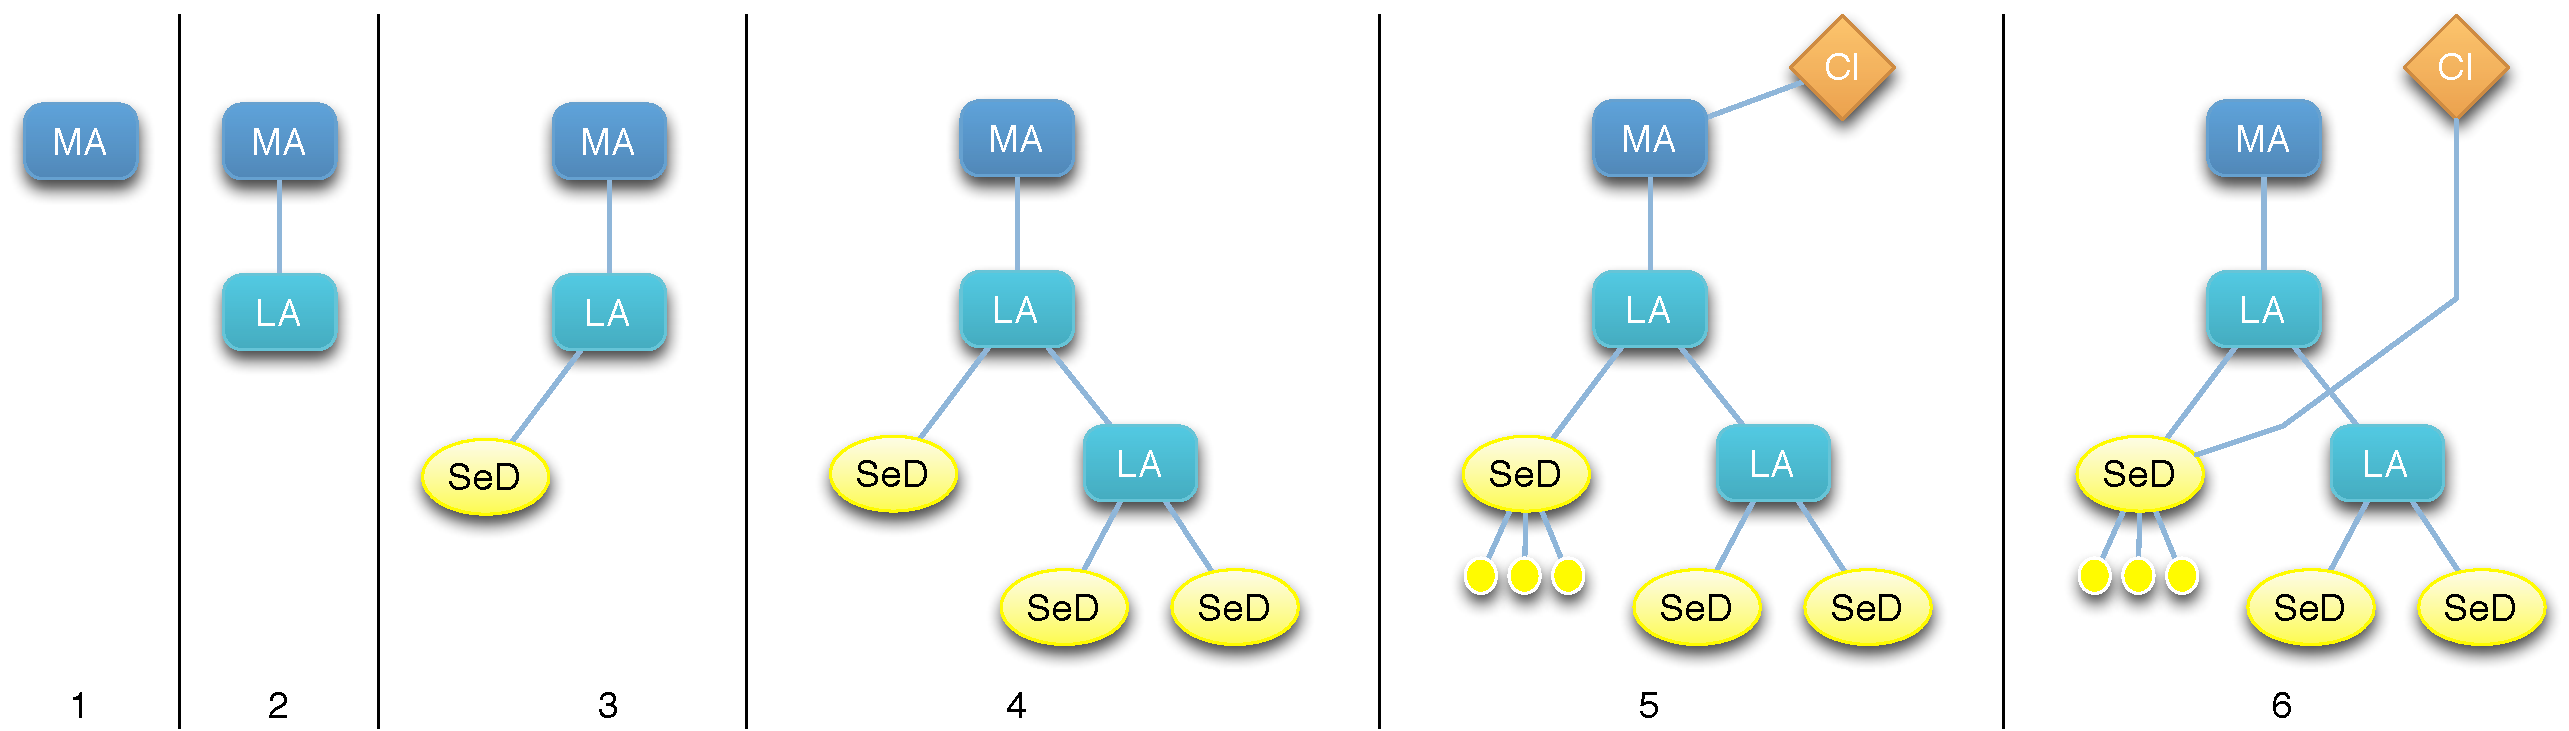
\includegraphics[scale=.6]{fig/init}
    \caption{Initialization of a \diet system.}
    \label{fig:init}
  \end{center}
\end{figure}

In step (2), an LA is launched and registers itself with the MA.
At this step of system initialization, two kinds of components can
connect to
the LA: a \sed ~(3), which manages some computational resource, or
another LA~(4), to add a hierarchical level in this branch. When the
\sed\ registers to its parent LA, it submits a list of the services it
offers.  The agent then reports the new service offering through its
parent agent until the MA.  If the service was previously unavailable
along that arm of the hierarchy the agents update their records.
Finally, clients can access the registered service by contacting
the MA~(5) to get a reference to the best server available and then
directly connect to it~(6) to launch the computation.

The architecture of the hierarchy is described in configuration files
(see Section~\ref{sec:diet_config_files})
and each component transmits the local configuration to its
parent. Thus, the system administration can also be hierarchical. For
instance, an MA can manage a domain like a university, providing
prioritary access to users of this domain. Then each laboratory can
run an LA, while each team of the laboratory can run some other LAs to
administrate its own servers. This hierarchical administration of the
system allows local changes in the configuration without interfering
with the whole platform.



%====[ Solving a problem ]=====================================================
\section{Solving a problem}
\label{sec:solvepb}

Assuming that the architecture described in Section
~\ref{sec:components} includes several servers able to solve the
same problem, the algorithm presented below lets an MA select a
server for the computation among those available. This decision is
made in four steps.

\begin{itemize}
\item The MA propagates the client request through its subtrees down
  to the capable servers; actually, the agents only forward the
  request on those subtrees offering the service.
\item Each server that can satisfy the request can send his 
  performance and hardware information or  an estimation of  the 
  computation time necessary to process the request to its ``parent'' (an LA)
  (via performance prediction tools: see Chapter~\ref{chapter:performance}). 
\item Each LA that receives one or more positive responses from its
  children sorts the servers and forwards the best responses to the MA
  through the hierarchy.
\item Once the MA has collected all the responses from its direct
  children, it chooses a pool of fast servers and sends their
  references to the client.
\end{itemize}

%====[ Extensions ]============================================================
\section{DIET Extensions}
\label{sec:extensions}

%====[ Multi-MA ]==============================================================
\subsection{Multi-MA}
\label{init:multima}

A standard \diet platform gives access to {\sed}s placed under the
control of a MA as explained at the beginning of this
chapter. Sometime, it is useful to connect several MA together. This
happens when several organizations wish to share their resources to
offer a larger set of service types and more available servers. The
Multi-MA extension allows this by creating a federation which shares
resources between several MA.

In multi-MA mode, the behavior of a \diet hierarchy does not change
when a client requests a service that is available under the queried
MA. However, if a request sent to a MA does not found a \sed that can
resolve its problem, \diet will forward the request to other MAs of
the federation.  To read more about multi-MA, see
Chapter~\ref{ch:multiMAextension} and Chapter~\ref{ch:p2pextension}.

%====[ FAST ]==============================================================
\subsection{FAST}
\label{sub:fast}

Fast Agent's System Timer (FAST)~\cite{Qui02} is a tool for dynamic
performance forecasting in a Grid environment.  When \diet is compiled
with the appropriate options and FAST has been configured on the \sed
machine, {\sed}s can access FAST to obtain dynamic performance
predictions.  See Chapter~\ref{chapter:performance} for details on
using FAST.

%====[ CoRI ]==============================================================
\subsection{CoRI}
\label{sub:cori}

Collector of Resource Information (CoRI) is a manager for collecting
hardware and performance information.  When \diet is compiled with the
appropriate option, it is possible to get this information via
different sub-modules like FAST* or CoRI-Easy. (* if compiled and
configured on the \sed machine). See Chapter~\ref{chapter:performance}
for details on using CoRI.

%%%%%%%%%%%%%%%
%% FIXME:
%%  Memory aspects should be treated here.
%%%%%%%%%%%%%%%

%%%%%%%%%%%%%%%
%% FIXME for DIET v1.1
%%%%%%%%%%%%%%%
% In order to solve the problem itself, the client connects to one of
% the servers chosen: it sends its local data and specifies if the
% results should be kept in-place for further computation or if they
% should be brought back. The transfer of persistent operands is
% performed at this stage.
%%%%%%%%%%%%%%%



%
% Installing
%
\newpage
%****************************************************************************%
%* DIET User's Manual installing chapter file                               *%
%*                                                                          *%
%*  Author(s):                                                              *%
%*    - Eddy CARON (Eddy.Caron@ens-lyon.fr)                                 *%
%*    - Pushpinder Kaur Chouhan (Pushpinder.Kaur.Chouhan@ens-lyon.fr)       *%
%*    - Philippe COMBES (Philippe.Combes@ens-lyon.fr)                       *%
%*                                                                          *%
%* $LICENSE$                                                                *%
%****************************************************************************%
%* $Id$
%* $Log$
%* Revision 1.11  2004/04/05 11:04:29  rbolze
%* add instruction to compile with logService
%*
%* Revision 1.10  2004/02/10 00:13:55  ecaron
%* Add bugzilla reference.
%*
%* Revision 1.9  2004/01/29 17:08:47  ecaron
%* Add suggestions from Frederic Desprez. Thanks !
%*
%* Revision 1.8  2004/01/21 23:23:03  ecaron
%* Add suggestions from Jean-Yves. Thanks !
%*
%* Revision 1.7  2004/01/21 00:25:13  ecaron
%* Add suggestions from Holly Dail. Thanks !
%*
%* Revision 1.6  2004/01/07 20:25:04  ecaron
%* Add ScaLAPACK and BLAS introduction
%*
%* Revision 1.5  2004/01/06 15:07:46  ecaron
%* Correct latex bug
%*
%* Revision 1.4  2003/12/12 14:42:44  pkchouha
%*  define \diet_version in UserManual.tex to be 1.0
%*
%* Revision 1.3  2003/12/03 11:06:57  pkchouha
%* 1. change the version of DIET to 1.0
%* 2. DIET.tgz to DIET_1.0.tgz
%* 3. added the unlisted options in  section 2.2.1
%* 4. commented the  all part of section 2.2.2 before the subcetion oniORB
%* 5. added the unlisted options in section 2.2.2
%* 6. changed the args to conftest.c -o conftest
%* 7. changed some words and sentances for simplification
%*
%* Revision 1.2  2003/11/28 11:51:36  pcombes
%* Correction about gcc-2.96 management of exception handling.
%*
%* Revision 1.1  2003/09/09 12:38:20  pcombes
%* Reorganization of doc: UM becomes UsersManual.
%*
%* Revision 1.12  2003/06/23 13:14:09  pcombes
%* Update example to new configuration summary.
%*
%* Revision 1.11  2003/06/16 17:39:55  pcombes
%* One word about gcc-2.96.
%*
%* Revision 1.10  2003/06/02 13:47:05  pcombes
%* Fix footnotesize.
%*
%* Revision 1.9  2003/05/23 09:23:35  pcombes
%* Add suggestions from Jean-Yves. Thanks !
%*
%* Revision 1.8  2003/05/15 14:17:58  pcombes
%* UM 0.7
%*
%* Revision 1.6  2003/01/24 16:58:54  pcombes
%* UM 0.6.4
%*
%* Revision 1.5  2003/01/22 17:34:53  pcombes
%* User Manual, v. 0.6.4
%****************************************************************************%


\chapter{DIET installation}
\label{ch:installing}

%====[ Dependencies ]==========================================================
\section{Dependencies}
\label{sec:dependencies}

\subsection{Hardware dependencies}

DIET has fully tested on Linux i386 and i686 platforms and has tested
on Solaris/Sparc, Linux/Sparc, Linux/i64 and Linux/Alpha platform and
seems be supported.

If you found a bug into DIET, please to submit a bug report at
\url{http://graal.ens-lyon.fr/bugzilla}. If you have multiple bugs to
report, please make multiple submissions, rather than submitting
multiple bugs in one report.

\subsection{Software dependencies}

As explained in Section \ref{sec:CORBA}, CORBA is used for all
communications inside the platform. So all of the three parts depend on it. The
implementations of CORBA currently supported in DIET are:
\begin{itemize}
 \item{\textbf{omniORB 3}} which depends on \textbf{Python 1.5}
 \item{\textbf{omniORB 4}} which depends on \textbf{Python 2.1} or later,
                           and on \textbf{OpenSSL} if you would like your DIET
                           platform to be secure.
% \item{soon \textbf{TAO 1.3}} which depends on \textbf{ACE} (but TAO is always
%                           provided with ACE)
\end{itemize}
We strongly recommend omniORB 4, as it is easier to install, and
provides SSL support. In order to deploy CORBA services with omniORB,
a configuration file and a log directory are required: see Section
\ref{sec:CORBA_services} for a complete description of the services.
Their path can be given to omniORB through environment variables
(\texttt{\$OMNIORB\_CONFIG} and \texttt{\$OMNINAMES\_LOGDIR}), and/or,
for \textbf{omniORB 4} only, at compile time, with the
\texttt{--with-omniORB-config} and \texttt{--with-omniNames-logdir}
options.

\noindent 
\textbf{NB:} We have noticed that some problems occur with \textbf{Python 2.3}:
the C++ code generated could not be compiled. It has been patched in DIET, but
some warnings still appear.
\\

Since omniORB needs a thread-safe management of exception handling, compiling
DIET with \verb+gcc+ requires at least \verb+gcc-2.96+.
\\

The agent and server parts of DIET can depend on FAST (see �\ref{sec:FAST}).
Although not absolutely compulsory, it is strongly recommended: indeed, all
communication and computation times are set to infinity if FAST is not
installed.  FAST depends on:
\begin{itemize}
 \item{\textbf{DB 2}} the Berkeley Database routines
 \item{\textbf{GSL}} the GNU Scientific Library
 \item{\textbf{OpenLDAP}} an implementation of the Lightweight Directory Access
                          Protocol
 \item{\textbf{NWS}} the Network Weather Service
\end{itemize}
For more details about FAST dependencies, please refer to the FAST
Reference
Manual~\footnote{\url{http://graal.ens-lyon.fr/FAST/docs}}.
It is important to understand basically how FAST works, and the role
of its dependencies, to deactivate the
ones that are not needed by the user.\\

Finally, some examples provided in the DIET sources depend on the BLAS
and \scalapack\ libraries. However theses examples do not have to be
compiled.


%====[ Compilation ]===========================================================
\section{Compiling the platform}
\label{sec:compil_platform}

Once all dependencies are satisfied, untar the DIET archive and
change to its root directory. A configure script will prepare DIET for
compiling: its main options are described below, but please, run
\texttt{configure --help} to get an up-to-date and complete usage description.\\

\noindent
{\footnotesize
\texttt{$\sim$> tar xzf DIET\_}\dietversion\texttt{.tgz} \\
\texttt{$\sim$> cd DIET} \\
\texttt{$\sim$/DIET> ./configure --help=short} \\
\texttt{Configuration of DIET} \dietversion \texttt{:} \\
\texttt{...}
}

\subsection{Optional features for configuration}

{\footnotesize
\begin{verbatim}
  --disable-FEATURE       do not include FEATURE (same as --enable-FEATURE=no)
  --enable-FEATURE[=ARG]  include FEATURE [ARG=yes]
  --enable-maintainer-mode enable make rules and dependencies not useful
                          (and sometimes confusing) to the casual installer
\end{verbatim}

\begin{verbatim}
  --enable-doc            enable the module doc, documentation about DIET
\end{verbatim}
}
\noindent This option activates the compilation and installation of the DIET
documents, which is disabled by default, because it is very sensitive to the
version of your \LaTeX\ compiler. The output postscript files are provided in
the archive.

{\footnotesize
\begin{verbatim}
  --disable-examples      disable the module examples, basic DIET examples
\end{verbatim}
}
\noindent This option deactivates the compilation of the DIET examples, which is
enabled by default.

{\footnotesize
\begin{verbatim}
  --enable-BLAS           enable the module BLAS, an example for calling BLAS
                          functions through DIET
\end{verbatim}
}
\noindent This option activates the compilation of the DIET BLAS examples, as a
sub-module of examples (which means that this option has no effect if examples
are disabled) - disabled by default.

{\footnotesize
\begin{verbatim}
  --enable-logservice     enable monitoring through LogService
\end{verbatim}
}
\noindent This option enables the connection from DIET to the LogService
monitoring software. It will enable DIET to generate monitoring data
and send it to the LogService. Note that the support of LogService is
built in. You do not have to install the LogService package to compile
with this option.

{\footnotesize
\begin{verbatim}
 --enable-ScaLAPACK      enable the module ScaLAPACK, an example for calling
                          ScaLAPACK functions through DIET
\end{verbatim}
}
\noindent This option activates the compilation of the DIET \scalapack\ examples,
as a sub-module of examples (which means that this option has no effect if
examples are disabled) - disabled by default.

{\footnotesize
\begin{verbatim}
  --enable-Cichlid        enable generation of communication logs for Cichlid
  --enable-stats          enable generation of statistics logs
  --enable-multi-MA       enable multi-MA architecture
  --disable-dependency-tracking Speeds up one-time builds
  --enable-dependency-tracking  Do not reject slow dependency extractors
  --enable-shared=PKGS    build shared libraries default=yes
  --enable-static=PKGS    build static libraries default=yes
  --enable-fast-install=PKGS optimize for fast installation default=yes
  --disable-libtool-lock  avoid locking (might break parallel builds)
\end{verbatim}
}

\begin{comment}
{\footnotesize
\begin{verbatim}
  --enable-multi-MA       enable multi-MA architecture
\end{verbatim}
}
\end{comment}


\subsection{Optional packages for configuration}


{\footnotesize
\begin{verbatim}
  --with-PACKAGE[=ARG]    use PACKAGE [ARG=yes]
  --without-PACKAGE       do not use PACKAGE (same as --with-PACKAGE=no)
  --with-gnu-ld           assume the C compiler uses GNU ld default=no
  --with-pic              try to use only PIC/non-PIC objects default=use both
\end{verbatim}
}

%% \subsubsection{The \texttt{--with-PKG-extra} option}

%% For all packages that DIET depends on, the \texttt{configure} script provides an
%% option that let the user define the arguments needed to compile with the
%% libraries of the package PKG: \texttt{--with-PKG-extra}. This is useful when
%% the \texttt{configure} script does not succeed on its own to get necessary
%% compilation option.

%% Let us take the example of a user who wishes to compile the BLAS examples (see
%% the BLAS subsection below). On the platform he/she uses, it is necessary to
%% specify the following arguments to compile with the BLAS library:

%% {\footnotesize \texttt{-lm -L/home/theuser/lib -lblas -lg2c -lm} }

%% \noindent
%% Let us assume that specifying the option
%% \texttt{--with-BLAS-libraries=/home/theuser/lib} is not enough for the
%% \texttt{configure} script to compile DIET examples. Then, the user will have to
%% add the following arguments to his/her \texttt{configure} command line:

%% {\footnotesize \texttt{--with-BLAS-extra="-lm -L/home/theuser/lib -lblas -lg2c
%%   -lm"} }

\subsubsection{omniORB}
{\footnotesize
\begin{verbatim}
  --with-omniORB=DIR      specify the root installation directory of omniORB
  --with-omniORB-includes=DIR
                          specify exact header directory for omniORB
  --with-omniORB-libraries=DIR
                          specify exact library directory for omniORB
  --with-omniORB-extra=ARG|"ARG1 ARG2 ..."
                          specify extra conftest.c -o conftest for the linker
                          to find the omniORB libraries (use "" in case of 
                          several conftest.c -o conftest)
\end{verbatim}
}
\noindent This group of options lets the user define all necessary paths to
compile with omniORB. Generally, \texttt{--with-omniORB=DIR} should be enough, and
the other options are provided for ugly installations of omniORB.\\
\textbf{NB:} having the executable \texttt{omniidl} in the PATH environment
variable should be enough in most cases.

\subsubsection{FAST}
{\footnotesize
\begin{verbatim}
  --with-FAST=DIR         installation root directory for FAST (optional)
  --with-FAST-bin=DIR     installation directory for fast-config (optional)
\end{verbatim}
}
\noindent This group of options lets the user define all necessary paths to
compile with FAST. Generally, \texttt{--with-FAST=DIR} should be enough, and the
other options are provided for difficult installations of FAST. There is no need to
specify includes, libraries and extra arguments, since FAST provides a tool
\texttt{fast-config} that does this job automatically.\\
\textbf{NB1:} having the executable \texttt{fast-config} in the PATH environment
variable should be enough in most cases.\\
\textbf{NB2:} it is possible to specify \texttt{--without-FAST}, which overrides
\texttt{fast-config} detection.

\subsubsection{BLAS}

The BLAS~\footnote{\url{http://www.netlib.org/blas/}} (Basic Linear
Algebra Subprograms) are high quality "building block" routines for
performing basic vector and matrix operations.  Level 1 BLAS do
vector-vector operations, Level 2 BLAS do matrix-vector operations,
and Level 3 BLAS do matrix-matrix operations. Because the BLAS are
efficient, portable, and widely available, they're commonly used in
the development of high quality linear algebra software.

{\footnotesize
\begin{verbatim}
  --with-BLAS=DIR  specify the root installation directory of BLAS (Basic
                   Linear Algebric Subroutines)

  --with-BLAS-includes=DIR
                   specify exact header directory for BLAS
  --with-BLAS-libraries=DIR
                   specify exact library directory for BLAS
  --with-BLAS-extra=ARG|"ARG1 ARG2 ..."
                   specify extra conftest.c -o conftest for the linker to find
                   the BLAS libraries (use "" in case of several 
                   conftest.c -o conftest)
\end{verbatim}
}
\noindent This group of options lets the user define all necessary paths to
compile with the BLAS libraries. Generally, \texttt{--with-BLAS=DIR} should be
enough, and the other options are provided for difficult installation of the BLAS.\\
\textbf{NB:} these options have no effect if the module example and/or its
sub-module BLAS are disabled.

\subsubsection{\scalapack}

The ScaLAPACK\footnote{\url{http://www.netlib.org/scalapack/}} (or
Scalable LAPACK) library includes a subset of LAPACK routines
redesigned for distributed memory MIMD parallel computers. It is
currently written in a Single-Program-Multiple-Data style using
explicit message passing for interprocessor communication. It assumes
matrices are laid out in a two-dimensional block cyclic decomposition.

Like LAPACK, the ScaLAPACK routines are based on block-partitioned
algorithms in order to minimize the frequency of data movements between
different levels of the memory hierarchy. (For such machines, the
memory hierarchy includes the off-processor memory of other
processors, in addition to the hierarchy of registers, cache, and
local memory on each processor.) The fundamental building blocks of
the ScaLAPACK library are distributed memory versions (PBLAS) of the
Level 1, 2 and 3 BLAS, and a set of Basic Linear Algebra Communication
Subprograms (BLACS) for communication tasks that arise frequently in
parallel linear algebra computations. In the ScaLAPACK routines, all
interprocessor communication occurs within the PBLAS and the BLACS.
One of the design goals of ScaLAPACK was to have the ScaLAPACK
routines resemble their LAPACK equivalents as much as possible.

For detailed information on ScaLAPACK, please refer to the ScaLAPACK
Users' Guide~\cite{BCC+97}.


{\footnotesize
\begin{verbatim}
  --with-ScaLAPACK=DIR    specify the root installation directory of ScaLAPACK
                          (parallel version of the LAPACK library)

  --with-ScaLAPACK-includes=DIR
                          specify exact header directory for ScaLAPACK
  --with-ScaLAPACK-libraries=DIR
                          specify exact library directory for ScaLAPACK
  --with-ScaLAPACK-extra=ARG|"ARG1 ARG2 ..."
                          specify extra conftest.c -o conftest for the linker to find 
                          the ScaLAPACK libraries (use "" in case of several 
                          conftest.c -o conftest)
\end{verbatim}
}

\noindent This group of options lets the user define all necessary paths for compilation with the \scalapack\ libraries. Normally, \texttt{--with-ScaLAPACK=DIR} could be enough, but the other options are provided because the
installation of the \scalapack\ libraries is often difficult, and thus
difficult to detect automatically. For instance, the
\texttt{--with-ScaLAPACK-extra} option is useful to integrate BLACS
and MPI libraries, which are useful for ScaLAPACK.
\\
\textbf{NB:} these options have no effect if the module example and/or
its sub-module \scalapack\ are disabled.


\subsection{From configuration to compilation}

An important option for configure scripts is \texttt{--prefix=}, which
specifies where binary files, documents and configuration files will
be installed. It is important to set this option: it otherwise
defaults to \texttt{DIET/install}.

The configuration will return with an error if no ORB was found. So please help
the configure script to find the ORB with the \texttt{--with-omniORB*} options.\\


If everything went OK, the configuration ends with a summary of the
options that were selected and what it was possible to get. The output
will look like: {\footnotesize
\begin{verbatim}
~/DIET > ./configure --enable-doc --enable-BLAS
DIET successfully configured as follows:
 - documents:       yes
 - examples:        dmat_manips, file_transfer, scalars
 - FAST:            found /home/username/DIET/FAST/bin/fast-config
 - ORB:             omniORB 4 in /usr
 - prefix:          /home/username/DIET/install
 - multi-MA:        no
 - target platform: i686-pc-linux-gnu
 
Please run make help to get compilation instructions.
~/DIET > make help
====================================================================
 Usage : make help     : shows this help screen
         make agent    : builds DIET agent executable
         make SeD      : builds DIET SeD library
         make client   : builds DIET client library
         make examples : builds basic examples
         make          : builds everything configured
         make install  : copy files into /home/username/DIET/install
====================================================================
\end{verbatim}
}

This helps the user to choose the DIET parts for installation and
compilation. It is recommended for beginners to compile the client,
the SeD and the agent in one single step with \texttt{make all}. But
please, pay attention to the fact that \texttt{make all} does not
install DIET in the prefix provided at configuration time. To do this,
run \texttt{make install}.

\texttt{make install} will run the compilation for all DIET entities before the
installation itself. Thus, if the user wants to compile only the agent, for
instance, and install it, he must run:
{\footnotesize
\begin{verbatim}
~/DIET > cd src/agent
~DIET/src/agent > make install
\end{verbatim}
}


\section{Compiling the examples}

Four series of examples are provided in the DIET archive:
\begin{itemize}
\item{\texttt{file\_transfer}}: the server computes the sizes of two
  input files and returns them. A third output parameter may be
  returned: randomly, the server decides to send back the first file.
  This is to show how to manage a variable number of arguments: the
  profile declares all arguments that may be filled, even if they
  might not be all filled at each request/computation.

\item{\texttt{dmat\_manips}}: the server offers matrix manipulation routines:
  transposition (\texttt{T}), product (\texttt{MatPROD}) and sum
  (\texttt{MatSUM}, \texttt{SqMatSUM} for square matrices, and
  \texttt{SqMatSUM\_opt} for square matrices but re-using the memory space of
  the second operand for the result). Any subset of these operations can be
  specified on the command line. The last two of them are given for
  compatibility with a BLAS server, explained below.
  
\item{\texttt{BLAS}}: the server offers the \texttt{dgemm} BLAS functionality.
  We plan to offer all BLAS (Basic Linear Algebric Subroutines) in the
  next DIET version. Since this function computes $C = \alpha AB +
  \beta C$, it can also compute a matrix-matrix product, a sum of
  square matrices, etc. All these services are offered by the BLAS
  server. Two clients are designed to use these services: one
  (\texttt{dgemm\_client.c}) is designed to use the \texttt{dgemm\_}
  function only, and the other one (\texttt{client.c}) to use all BLAS
  functions (but currently only \texttt{dgemm\_}) and sub-services,
  such as \texttt{MatPROD}.
  
\item{\texttt{\scalapack}}: the server is designed to offer all \scalapack\ 
  (parallel version of the LAPACK library) functions but only manages the
  \texttt{pdgemm\_} function so far. The \texttt{pdgemm\_} routine is the
  parallel version of the \texttt{dgemm\_} function, so that the server also
  offers all the same sub-services. Two clients are designed to use these
  services: one (\texttt{pdgemm\_client.c}) is designed to use the
  \texttt{pdgemm\_} function only, and the other one (\texttt{client.c}) to use
  all \scalapack\ functions and sub-services, such as \texttt{MatPROD}.
\end{itemize}

Running \texttt{make install} in the \texttt{examples} directory (or in the root
directory, when DIET is configured with \texttt{--enable-examples}) does not
copy binary files into \texttt{$<$install\_dir$>$/bin}, but in
\texttt{examples/bin}: this odd behaviour is due to some limitations of the
\textsf{automake} tool.

Likewise, the samples of configuration files located in
\texttt{examples/cfgs} are processed by \texttt{make install} to
create ready-to-use configuration files in \texttt{examples/etc} and
then copied into \texttt{$<$install\_dir$>$/etc}. Successive calls to
make install will not erase the configuration files created and copied
the first time, except if \texttt{make uninstall} is called inbetween ;
thus the user will not lose the changes to these files.



%
% DIET data
%
\newpage
%****************************************************************************%
%* DIET User's Manual data chapter file                                     *%
%*                                                                          *%
%*  Author(s):                                                              *%
%*    - Philippe COMBES (Philippe.Combes@ens-lyon.fr)                       *%
%*                                                                          *%
%* $LICENSE$                                                                *%
%****************************************************************************%
%* $Id$
%* $Log$
%* Revision 1.20  2006/12/05 09:11:29  rbolze
%* some corrections
%*
%* Revision 1.19  2006/06/30 15:47:41  ycaniou
%* Coquilles, and batch stuff
%*
%* Revision 1.18  2005/07/13 09:37:39  ecaron
%* Remove fixme Bruno
%*
%* Revision 1.17  2005/07/12 21:44:28  hdail
%* - Correcting small problems throughout
%* - Modified deployment chapter to have a real section for deploying via GoDIET
%* - Adding short xml example without the comments to make a figure in GoDIET
%*   section.
%*
%* Revision 1.16  2005/07/12 09:11:32  ecaron
%* Fix free matrices memory
%*
%* Revision 1.15  2005/07/12 08:00:03  ecaron
%* Swap Schedulin in DIET and FAST section
%*
%* Revision 1.14  2005/06/27 08:32:52  hdail
%* fixme for addition of free for user-defined and out parameters at end of sample
%* code segments.
%*
%* Revision 1.13  2005/06/27 07:55:06  hdail
%* Correcting english etc.  Added some fixmes where I didn't know how to correct
%* old text.
%*
%* Revision 1.12  2005/06/14 08:16:06  ecaron
%* Typo
%*
%* Revision 1.11  2005/04/22 10:35:53  ycaniou
%* The fourth arg of diet_string_set(), size_t length, does not exist
%*
%* Revision 1.10  2004/08/27 17:04:36  ctedesch
%* - update DIET J chapter :
%* use of the PIF DIET
%* JXTA -> DIET J
%*
%* - syntax corrections in data chapter (_ -> \_)
%*
%* Revision 1.9  2004/07/20 08:34:20  bdelfabr
%* corrections. Thanks Matthias.
%*
%* Revision 1.8  2004/07/01 08:53:10  bdelfabr
%* add data management part in section 3.
%*
%* Revision 1.7  2004/02/10 01:58:08  ecaron
%* Add suggesstions from Matthias Colin. Thanks!
%*
%* Revision 1.6  2004/02/10 00:38:25  ecaron
%* Add suggestions from Jean-Yves L'Excellent. Thanks !
%****************************************************************************%

\chapter{DIET data}
\label{ch:data}

It is important that DIET can manipulate data to optimize copies and
memory allocation, to estimate data transfer and computation time,
etc. Therefore the data must be fully described in terms of their data 
types and various attributes associated with these types.

\section{Data types}
\label{sec:types}

DIET defines a precise set of data types to be used to describe the arguments of
the services (on the server side) and of the problems (on the client side).

The DIET data types are defined in the file
\texttt{$<$install\_dir$>$/include/DIET\_data.h}. The user will also find in
this file various function prototypes to manipulate all DIET data types. Please
refer to this file for a complete and up-to-date API description.

To keep DIET type descriptions generic, two main sets are used: base and
composite types.

\subsection{Base types}
\label{ssec:base}

Base types are defined in an enum type \texttt{diet\_base\_type\_t} and have the
following semantics:
\begin{center}
\footnotesize
\begin{tabular}{|l|l|c|}
\hline
\textbf{Type}&\textbf{Description}&\textbf{Size in octets}\\
\hline
\textsf{DIET\_CHAR}     & Character                &  1\\
\textsf{DIET\_BYTE}     & Octet                    &  1\\
\textsf{DIET\_INT}      & Signed integer           &  4\\
\textsf{DIET\_LONGINT}  & Long signed integer      &  8\\
\textsf{DIET\_FLOAT}    & Simple precision real    &  4\\
\textsf{DIET\_DOUBLE}   & Double precision real    &  8\\
\hline\hline
\textsf{DIET\_SCOMPLEX} & Simple precision complex &  8\\
\textsf{DIET\_DCOMPLEX} & Double precision complex & 16\\
\hline
\end{tabular}
\end{center}

\begin{itemize}
\item[NB:] \textsf{DIET\_SCOMPLEX} and \textsf{DIET\_DCOMPLEX} are not implemented yet.
\end{itemize}


\subsection{Composite types}
\label{ssec:complex}

Composite types are defined in an enum type \texttt{diet\_type\_t}:
\begin{center}
\footnotesize
\begin{tabular}{|l|l|}
\hline
\textbf{Type}&\textbf{Possible base types}\\
\hline
\textsf{DIET\_SCALAR} & all base types\\
\textsf{DIET\_VECTOR} & all base types\\
\textsf{DIET\_MATRIX} & all base types\\
\textsf{DIET\_STRING} & \textsf{DIET\_CHAR}\\
\textsf{DIET\_FILE}   & \textsf{DIET\_CHAR}\\
\hline
\end{tabular}
\end{center}

Each of these types requires specific parameters to completely describe the
data (see Figure \ref{fig:data}).


\subsection{Persistence mode}
\label{ssec:persismode}
Persistence mode is defined in an enum type \texttt{diet\_persistence\_mode\_t}

\begin{center}
\footnotesize
\begin{tabular}{|l|l|}
\hline
\textbf{mode}&\textbf{Description}\\
\hline
\textsf{DIET\_VOLATILE} & not stored\\
\textsf{DIET\_PERSISTENT\_RETURN} & stored on server, movable and copy back to client\\
\textsf{DIET\_PERSISTENT} & stored on server and movable\\
\textsf{DIET\_STICKY} & stored and non movable\\
\hline\hline
\textsf{DIET\_STICKY\_RETURN} & stored, non movable and copy back to client\\
\hline
\end{tabular}
\end{center}

\begin{itemize}
\item[NB:] \textsf{DIET\_STICKY\_RETURN} is not implemented yet.
\end{itemize}

\section{Data description}
\label{sec:datadesc}

Each parameter of a client problem is manipulated by DIET using the following
structure:
{\footnotesize
\begin{verbatim}
typedef struct diet_arg_s diet_arg_t;
struct diet_arg_s{
  diet_data_desc_t desc;
  void            *value;
};
typedef diet_arg_t diet_data_t;
\end{verbatim}
}

The second field is a pointer to the memory zone where the parameter data are
stored. The first one consists of a complete DIET data description, which is
better described by a figure than with C code, since it can be set and accessed
through API functions. Figure \ref{fig:data} shows the data classification used
in DIET. Every ``class'' inherits from the root ``class'' \texttt{data}, and
could also be a parent of more detailed classes of data in future versions of
DIET.

\begin{figure}[hpt]
 \begin{center}
  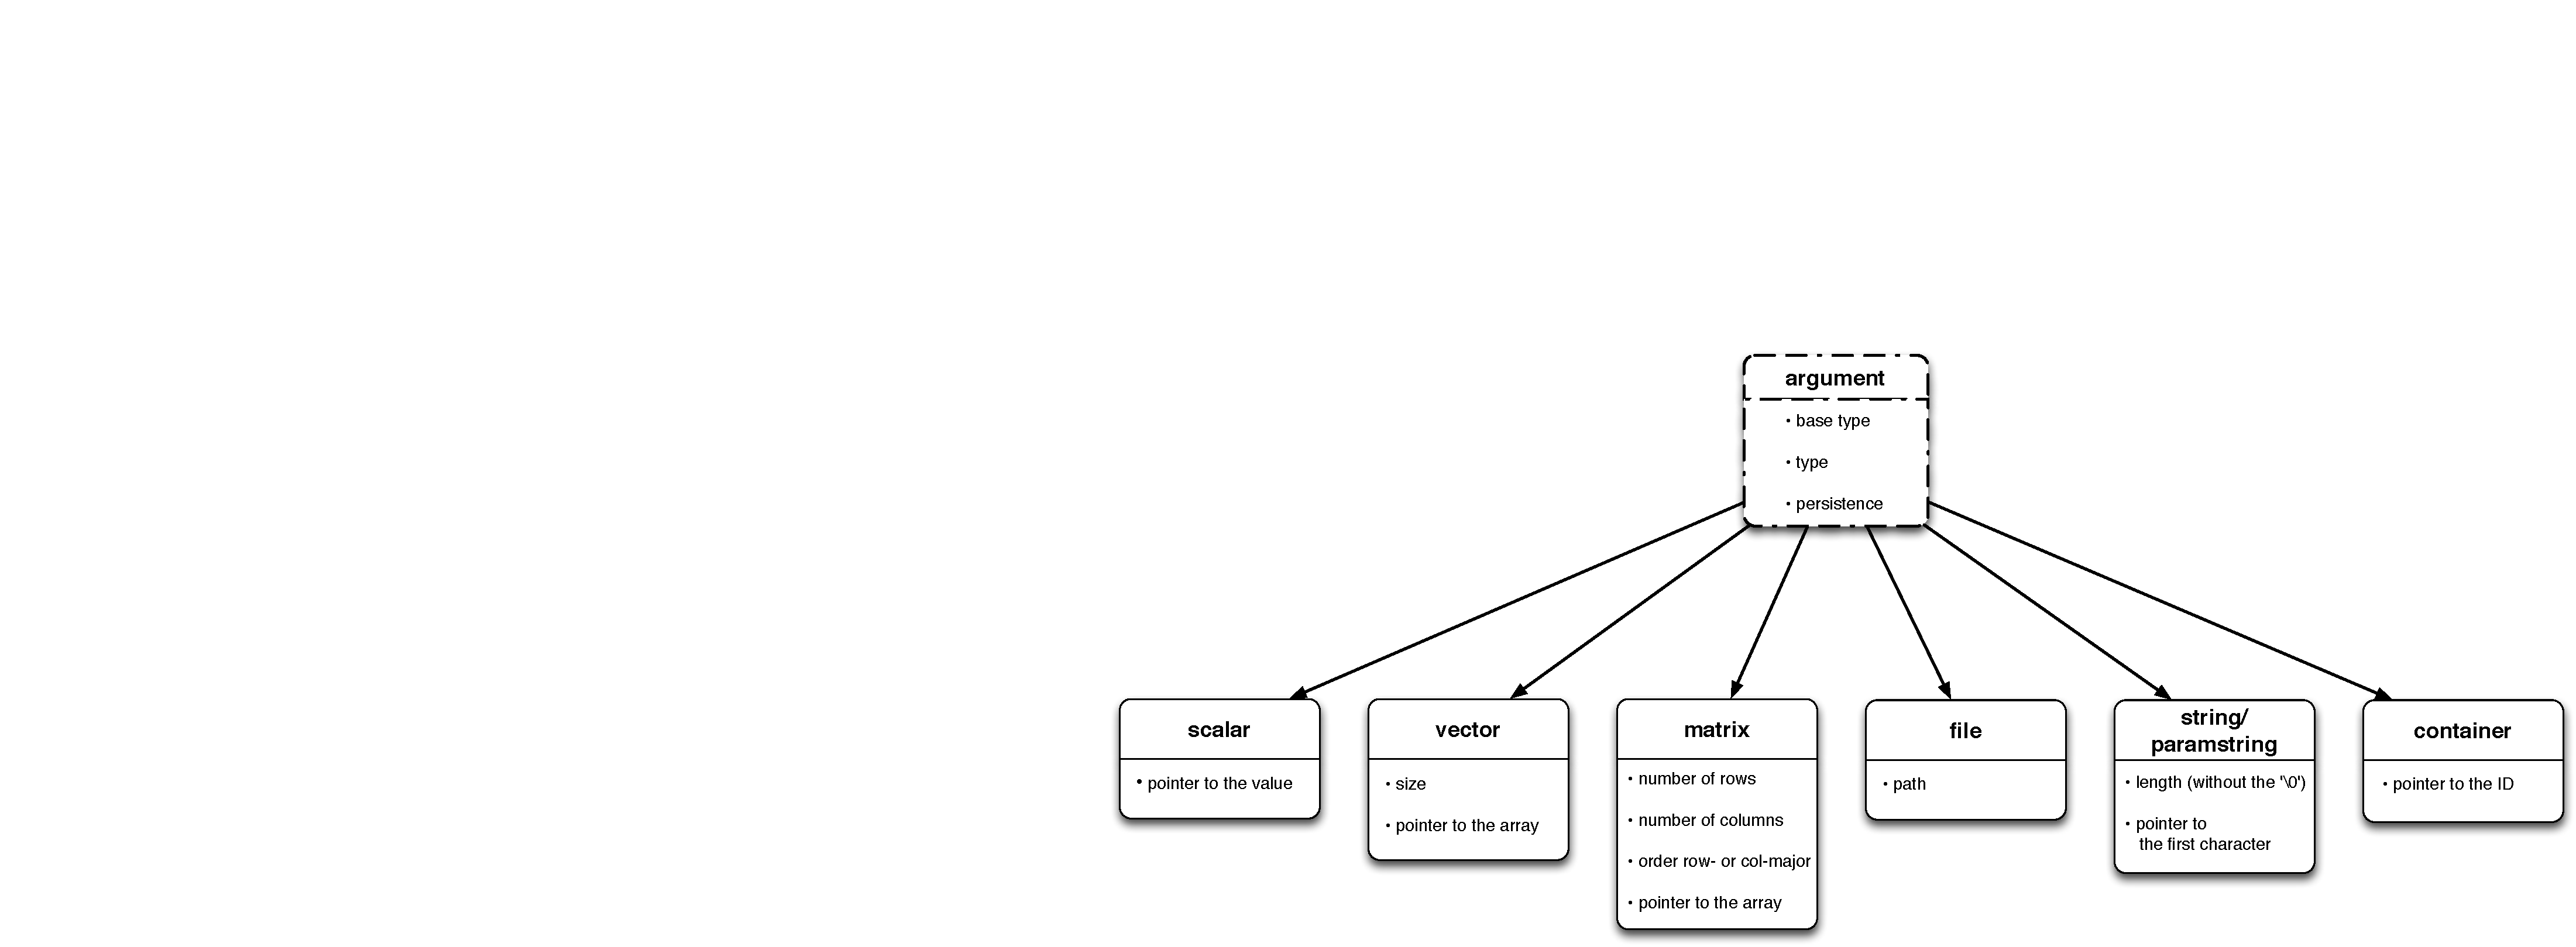
\includegraphics[scale=.5]{fig/data.eps}
  \caption{Argument/Data structure description.}
  \label{fig:data}
 \end{center}
\end{figure}


\section{Data management}
\label{sec:datamgt}

\subsection{Data identifier}
\label{ssec:dataid}
The data identifier is generated by the MA. The data identifier is a
string field that contains the MA name, the number of the session plus
the number of the data in the problem (incremental) plus the string
``id''.  This is the \texttt{id} field of the
\texttt{diet\_data\_desc\_t} structure.

{\footnotesize
\begin{verbatim}
typedef struct {
  char* id;  
  diet_persistence_mode_t  mode;
  ....
} diet_data_desc_t;
\end{verbatim}
}

For example, \textbf{id.MA1.1.1} will identify the first data
in the first session submitted on the Master Agent \textbf{MA1}.


\begin{itemize}
\item[NB:] the field ``id'' of the identifier will be next replaced by a
client identifier. This is not implemented yet.
\end{itemize}

\subsection{Data file}
\label{ssec:datafile}

The name of the file is generated by a Master Agent. It is created
during the \texttt{diet\_initialize()} call. The name of the file is
the aggregation of the string ID\_FILE plus the name of the MA plus
the number of the session.  

A file is created only when there are some persistent data in the
session.  

For example, \textbf{ID\_FILE.MA1.1} means the identifiers
of the persistent data stored are in the file corresponding to the
first session in the Master Agent \textbf{MA1}.

The file is stored in the \texttt{/tmp} directory.

\begin{itemize}
\item[NB:] for the moment, when a data item is erased from the platform, the
file isn't updated.
\end{itemize}


\section{Manipulating DIET structures}
\label{sec:manip}

The user will notice that the API to the DIET data structures consists of
modifier and accessor functions only: no allocation function is required, since
\texttt{diet\_profile\_alloc} (see Section \ref{sec:pbdesc}) allocates all
necessary memory for all argument \textbf{descriptions}. This avoids the
temptation for the user to allocate the memory for these data structures twice
(which would lead to DIET errors while reading profile arguments). Please see
the example in Section \ref{sec:pbex} for a typical use.
\\

Moreover, the user should know that arguments of the \texttt{\_set} functions
that are passed by pointers are \textbf{not} copied, in order to save memory.
This is true for the \emph{value} arguments, but also for the \emph{path} in
\texttt{diet\_file\_set}. Thus, the user keeps ownership of the memory zones
pointed at by these pointers, and he/she must be very careful not to alter it
during a call to DIET.

\subsection{Set functions}

%The data persistence is not available in this current
%version~\footnote{the data persistence will be available in DIET
%  v1.1}, thus fix the mode of the diet persistence parameter to 0.

\label{sec:setfun}
{\footnotesize
\begin{verbatim}
/**
 * On the server side, these functions should not be used on arguments, but only
 * on convertors (see section 5.5).
 * If mode                                is DIET_PERSISTENCE_MODE_COUNT, 
 * or if base_type                        is DIET_BASE_TYPE_COUNT,
 * or if order                            is DIET_MATRIX_ORDER_COUNT,
 * or if size, nb_rows, nb_cols or length is 0,
 * or if path                             is NULL,
 * then the corresponding field is not modified.
 */

int
diet_scalar_set(diet_arg_t* arg, void* value, diet_persistence_mode_t mode,
                diet_base_type_t base_type);
int
diet_vector_set(diet_arg_t* arg, void* value, diet_persistence_mode_t mode,
                diet_base_type_t base_type, size_t size);

/* Matrices can be stored by rows or by columns */
typedef enum {
  DIET_COL_MAJOR = 0,
  DIET_ROW_MAJOR,
  DIET_MATRIX_ORDER_COUNT
} diet_matrix_order_t;

int
diet_matrix_set(diet_arg_t* arg, void* value, diet_persistence_mode_t mode,
                diet_base_type_t base_type,
                size_t nb_rows, size_t nb_cols, diet_matrix_order_t order);
int
diet_string_set(diet_arg_t* arg, char* value, diet_persistence_mode_t mode);

/* The file size is computed and stocked in a field of arg
   ! Warning ! The path is not duplicated !!! */
int
diet_file_set(diet_arg_t* arg, diet_persistence_mode_t mode, char* path);
\end{verbatim}
}


\subsection{Access functions}
\label{sec:accessfun}
{\footnotesize
\begin{verbatim}
/**
 * A NULL pointer is not an error (except for arg): it is simply IGNORED.
 * For instance,
 *   diet_scalar_get(arg, &value, NULL),
 * will only set the value to the value field of the (*arg) structure.
 * 
 * NB: these are macros that let the user not worry about casting (int **)
 * or (double **) etc. into (void **).
 */

/**
 * Type: int diet_scalar_get((diet_arg_t *), (void *),
 *                           (diet_persistence_mode_t *))
 */
#define diet_scalar_get(arg, value, mode) \
        _scalar_get(arg, (void *)value, mode)
/**
 * Type: int diet_vector_get((diet_arg_t *), (void **),
 *                           (diet_persistence_mode_t *), (size_t *))
 */
#define diet_vector_get(arg, value, mode, size) \
        _vector_get(arg, (void **)value, mode, size)
/**
 * Type: int diet_matrix_get((diet_arg_t *), (void **),
 *                           (diet_persistence_mode_t *),
 *                           (size_t *), (size_t *), (diet_matrix_order_t *))
 */
#define diet_matrix_get(arg, value, mode, nb_rows, nb_cols, order) \
        _matrix_get(arg, (void **)value, mode, nb_rows, nb_cols, order)
/**
 * Type: int diet_string_get((diet_arg_t *), (char **),
 *                           (diet_persistence_mode_t *))
 */
#define diet_string_get(arg, value, mode, length) \
        _string_get(arg, (char **)value, mode)
/**
 * Type: int diet_file_get((diet_arg_t *),
 *                         (diet_persistence_mode_t *), (size_t *), (char **))
 */
#define diet_file_get(arg, mode, size, path) \
        _file_get(arg, mode, size, (char **)path)
\end{verbatim}
}


\section{Data Management functions}

\begin{itemize}
\item {The \texttt{store\_id} method} is used to store the
identifier of persistent data. It also accepts a description of
the data stored. This method has to be called after the
\texttt{diet\_call()}
\begin{verbatim}
  store_id(char* argID,char *msg);
\end{verbatim}

\item The \texttt{diet\_use\_data} method allows the client to use a data
item that is already stored in the platform.
\begin{verbatim}
  diet_use_data(diet_arg_t* arg,char* argID);
\end{verbatim}
This function replaces the set functions (see Section \ref{sec:setfun}).



\begin{itemize}
\item[NB:] a mechanism for data identifier publication hasn't been 
implemented yet. So, exchanges of identifiers between end-users that
want to share data must be done explicitly.
\end{itemize}



\item {The \texttt{diet\_free\_persistent\_data} method} allows the
client to remove a persistent data item from the platform.
\begin{verbatim}
  diet_free_persistent_data(char *argID);
\end{verbatim}

\end{itemize}


{\footnotesize
\begin{verbatim}

/*******************************************************************
 *   Add handler argID and text message msg in the identifier file *
 ******************************************************************/

void 
store_id(char* argID, char* msg);


/** sets only identifier : data is present inside the platform */

void
diet_use_data(diet_arg_t* arg, char* argID);


/******************************************************************
 *  Free persistent data identified by argID                     *
 *****************************************************************/
int
diet_free_persistent_data(char* argID);

\end{verbatim}
}


\subsection{Free functions}
\label{sec:freefun}

The amount of data  pointed at by value fields should be freed through a DIET
API function:
{\footnotesize
\begin{verbatim}
/****************************************************************************/
/* Free the amount of data pointed at by the value field of an argument.    */
/* This should be used ONLY for VOLATILE data,                              */
/*    - on the server for IN arguments that will no longer be used          */
/*    - on the client for OUT arguments, after the problem has been solved, */
/*      when they will no longer be used.                                   */
/* NB: for files, this function removes the file and frees the path (since  */
/*     it has been dynamically allocated by DIET in both cases)             */
/****************************************************************************/

int
diet_free_data(diet_arg_t* arg);
\end{verbatim}
}


\section{Problem description}
\label{sec:pbdesc}

For DIET to match the client problem with a service, servers and clients must
``speak the same language'', \emph{ie} they must use the same problem
description. A unified way to describe problems is to use a name and define its
profile with the type \texttt{diet\_profile\_t}:
{\footnotesize
\begin{verbatim}
typedef struct {
  int         last_in, last_inout, last_out;
  diet_arg_t *parameters;
} diet_profile_t;
\end{verbatim}
}

%%% \fixme{FIXME:
%%% as soon as persistency is integrated, this should become the table Eddy
%%% prepared to explain the transfer policy, depending on the modes.}


The field \emph{parameters} consists of a \texttt{diet\_arg\_t} array of size
$last\_out + 1$. Arguments can be
\begin{description}
\item{IN:}    The data are sent to the server. The memory is allocated
  by the user.
\item{INOUT:} The data are allocated by the user as for the IN
  arguments, then sent to the server and brought back into the same memory zone
  after the computation has completed, without any copy. Thus freeing this
  memory at the client while the computation is performed on the
  server would result in a segmentation fault when the data are
  brought back onto the client.
\item{OUT:} The data are created on the server and brought back into a
  newly allocated zone on the client. This allocation is performed by
  DIET. After the call has returned, the user can find the result in
  the zone pointed at by the \emph{value} field. Of course, DIET
  cannot guess how long the user will need these data, so the
  user must free the memory him/herself with \texttt{diet\_free\_data}.
\end{description}

%\fixme{This behaviour will be modified soon with the introduction of the
%persistence modes that will let the user leave some data on the
%servers for later computations.}

The fields \emph{last\_in}, \emph{last\_inout} and \emph{last\_out} of the
\texttt{diet\_profile\_t} structure respectively point at the indexes in the
\emph{parameters} array of the last IN, INOUT and OUT arguments.

Functions to create and destroy such profiles are defined with the prototypes
below:
{\footnotesize
\begin{verbatim}
diet_profile_t *diet_profile_alloc(int last_in, int last_inout, int last_out);
int diet_profile_free(diet_profile_t *profile);
\end{verbatim}
}



\section{Examples}
\label{sec:pbex}

\subsection{Example 1: without persistency}
Let us consider the product of a scalar by a matrix: the matrix must be
multiplied in-place, and the computation time must be returned.  This
problem has one IN argument (the scalar factor), one INOUT argument (the matrix)
and one OUT argument (the computation time), so its profile will be built as
follows:
\begin{center}
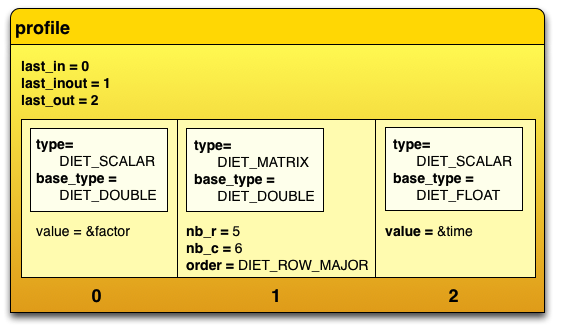
\includegraphics[scale=.35]{fig/smprod.eps}
\end{center}

Here are the lines of C code to generate such a profile:
{\footnotesize
\begin{verbatim}
  double  factor;
  double *matrix;
  float  *time;
  // Init matrix at least, factor and time too would be better ...
  // ...
  diet_profile_t profile = diet_profile_alloc(0, 1, 2); // last_in, last_inout, last_out
  diet_scalar_set(diet_parameter(profile,0), &factor, 0, DIET_DOUBLE);
  diet_matrix_set(diet_parameter(profile,1), matrix,  0, DIET_DOUBLE, 5, 6, DIET_ROW_MAJOR);
  diet_scalar_set(diet_parameter(profile,2), NULL,    0, DIET_FLOAT);
\end{verbatim}
}

\begin{itemize}
\item[NB1:] If there is no IN argument, \emph{last\_in} must be set to
  -1, if there is no INOUT argument, \emph{last\_inout} must
  be equal to \emph{last\_in}, and if there is no OUT argument,
  \emph{last\_out} must be equal to \emph{last\_inout}.
\item[NB2:] The \emph{value} argument for \texttt{\_set} functions
  (\ref{sec:setfun}) is ignored for OUT arguments, since DIET
  allocates the necessary memory space when the corresponding data are
  transferred from the server, so set value to NULL.
\end{itemize}

\subsection{Example 2: using persistency}

Let us consider the following problem : $C=A*B$, with A,B and C
persistent matrices.


{\footnotesize
\begin{verbatim}
  double *A, *B, *C; 
  // matrices initialization
  ...
  diet_initialize();
  strcpy(path,"MatPROD");
  profile = diet_profile_alloc(path, 1, 1, 2);
  diet_matrix_set(diet_parameter(profile,0),
                  A, DIET_PERSISTENT, DIET_DOUBLE, mA, nA, oA);
  print_matrix(A, mA, nA, (oA == DIET_ROW_MAJOR));
  diet_matrix_set(diet_parameter(profile,1),
                  B, DIET_PERSISTENT, DIET_DOUBLE, mB, nB, oB);
  print_matrix(B, mB, nB, (oB == DIET_ROW_MAJOR));
  diet_matrix_set(diet_parameter(profile,2),
                  NULL, DIET_PERSISTENT_RETURN, DIET_DOUBLE, mA, nB, oC);
  
  if (!diet_call(profile)) {
    diet_matrix_get(diet_parameter(profile,2),&C, NULL, &mA, &nB, &oC);
    store_id(profile->parameters[2].desc.id,"matrix C of doubles");
    store_id(profile->parameters[1].desc.id,"matrix B of doubles");
    store_id(profile->parameters[0].desc.id,"matrix A of doubles");
    print_matrix(C, mA, nB, (oC == DIET_ROW_MAJOR));
      
  }
  diet_profile_free(profile);
  // free matrices memory
  ...
  diet_finalize();
\end{verbatim}
}

Then, a client submits the problem : $D=E+C$ with C already present
in the platform. We consider that the handle of C is ``id.MA1.1.3''.

{\footnotesize
\begin{verbatim}
  double *C, *D, *E; 
  // matrices initialization
  ...
  diet_initialize();

  strcpy(path,"MatSUM");
  profile2 = diet_profile_alloc(path, 1, 1, 2);
  
  printf("second pb\n\n");
  diet_use_data(diet_parameter(profile2,0), "id.MA1.1.3");
  diet_matrix_set(diet_parameter(profile2,1),
                  E, DIET_PERSISTENT, DIET_DOUBLE, mA, nB, oE);
  print_matrix(E, mA, nB, (oE == DIET_ROW_MAJOR));
  diet_matrix_set(diet_parameter(profile2,2),
                  NULL, DIET_PERSISTENT_RETURN, DIET_DOUBLE, mA, nB, oD);
  
  if (!diet_call(profile2)) {
   diet_matrix_get(diet_parameter(profile2,2), &D, NULL, &mA, &nB, &oD);
   print_matrix(D, mA, nB, (oD == DIET_ROW_MAJOR));
   store_id(profile2->parameters[2].desc.id,"matrix D of doubles");
   store_id(profile2->parameters[1].desc.id,"matrix E of doubles");
  
  }
  diet_profile_free(profile2);
  diet_free_persistent_data("id.MA1.1.3");
  // free matrices memory
  ...
  diet_finalize();
\end{verbatim}
}  

Note that when a single client creates persistent data with a first
DIET call and uses that data with a second DIET call, we will not
know in advance the identifier of the data.  However, the identifier 
is stored in the structure of the first profile. For example,
consider a matrix A built with
\texttt{diet\_matrix\_set()} method as follows: {\footnotesize
\begin{verbatim}
  ...
  diet_profile_t *profile;
  ...
  diet_matrix_set(diet_parameter(profile,0),
                  E, DIET_PERSISTENT, DIET_DOUBLE, mA, nA, oA);
  ...
\end{verbatim}
} After the first \texttt{diet\_call}, the identifier of A is stored in
the profile (in \texttt{profile->parameters[0].desc.id}). So, for the
second call we will have the following instruction in order to use A:
{\footnotesize
\begin{verbatim}
  ...
  diet_profile_t *profile2;
  ...
  diet_use_data(diet_parameter(profile2,0),profile->parameters[0].desc.id);
  ...
\end{verbatim}
}

\begin{itemize}
\item[NB:] when using this method, the first profile (here
\texttt{profile}) must not be freed before using or making a copy of
the data identifier.
\end{itemize}


%
% Building a client program
%
\newpage
%****************************************************************************%
%* DIET User's Manual client chapter file                                   *%
%*                                                                          *%
%*  Author(s):                                                              *%
%*    - Philippe COMBES (Philippe.Combes@ens-lyon.fr)                       *%
%*                                                                          *%
%* $LICENSE$                                                                *%
%****************************************************************************%
%* $Id$
%* $Log$
%* Revision 1.2  2003/12/12 12:36:17  ecaron
%* Change call to diet_initialize()
%* Correct some bug
%*
%* Revision 1.1  2003/09/09 12:38:20  pcombes
%* Reorganization of doc: UM becomes UsersManual.
%*
%* Revision 1.11  2003/06/02 13:47:05  pcombes
%* Fix footnotesize.
%*
%* Revision 1.10  2003/05/23 09:23:35  pcombes
%* Add suggestions from Jean-Yves. Thanks !
%*
%* Revision 1.9  2003/05/15 14:17:58  pcombes
%* UM 0.7
%*
%* Revision 1.6  2003/01/24 16:58:54  pcombes
%* UM 0.6.4
%*
%* Revision 1.4  2003/01/21 12:17:02  pcombes
%* Update UM to API 0.6.3, and "hide" data structures.
%*
%* Revision 1.3  2003/01/14 08:04:36  pcombes
%* MAJ
%*
%* Revision 1.2  2003/01/13 12:09:00  pcombes
%* UM: client part complete for users's day ...
%****************************************************************************%

\chapter{Building a client program}
\label{ch:client}

The most difficult in building a client program is to understand the way a
problem has to be described. Once this first step is done, it is fairly easy to
build the successive calls to DIET.


\section{Structure of the program}
\label{sec:cl_struct}

Since the client side of DIET is a library, a client program has to define the
\texttt{main} function: it uses DIET through function calls. The complete
client-side interface is described in the \texttt{$<$install\_dir$>$/include}
files \texttt{DIET\_data.h} (see Chapter \ref{ch:data}) and
\texttt{DIET\_client.h}. So please refer to these two files for a complete and
up-to-date API description, and include at least the latter at the beginning of
your source code (\texttt{DIET\_client.h} includes \texttt{DIET\_data.h}):
{\footnotesize
\begin{verbatim}
#include <stdio.h>
#include <stdlib.h>

#include "DIET_client.h"

int main(int argc, char *argv[])
{
  diet_initialize(configuration_file, argc, argv);
  // Successive DIET calls ...
  diet_finalize();
}
\end{verbatim}
}

The client program must open its DIET session with a call to
\texttt{diet\_initialize}, which parses the configuration file to set
all options and get a reference to the DIET Master Agent. The session
is closed with a call to \texttt{diet\_finalize}, which aims at
freeing all resources, if any, associated to this session on the
client, servers, and agents, but not the memory allocated for
all INOUT and OUT arguments brought back onto the client during the
session, so that the user can still access them (and still have to
free them !)


\section{Client API}
\label{sec:clAPI}

The client API follows the GridRPC definition \cite{gridRPC:02}: all
\texttt{diet\_} functions are ``duplicated'' with \texttt{grpc\_}
functions.  Both \texttt{diet\_initialize} and \texttt{diet\_finalize}
belong to the GridRPC API.  One important thing to notice is that the
GridRPC defines an asynchronous API that is not fully implemented in
DIET yet (it is redirected onto the synchronous API). \fixme{check with CP} \\

A problem is managed through a \emph{function\_handle}, that associates a server
to a problem name. Please do not use \texttt{diet\_function\_handle\_init},
since it assumes that the client already knows the server, and DIET is not
conceived for such a use.. This function is only provided for GridRPC
compliance. The structure allocation is performed through the function
\texttt{diet\_function\_handle\_default}.

The \emph{function\_handle} returned is associated to the problem description,
its profile, in the call to \texttt{diet\_call}.

\section{Example}
\label{sec:cl_ex}

Let us consider the same example as in Section \ref{sec:pbex}.  Here, the client
configuration file is given as the first argument on the command line, and we
decide to hardcode the matrix, its factor, and the name of the problem:
\texttt{smprod}~\footnote{Source code available \texttt{doc/tutorial/solutions/exercise2/client_smprod.c}} for scalar by matrix product.


{\footnotesize
\begin{verbatim}
#include <stdio.h>
#include <stdlib.h>
#include <math.h>
#include "DIET_client.h"

int main(int argc, char **argv)
{
  int i;
  double  factor = M_PI; /* Pi, why not ? */
  double *matrix;        /* The matrix to multiply */
  float  *time   = NULL; /* To check that time is set by the server */

  diet_function_handle_t *fhandle;
  diet_profile_t         *profile;

  /* Allocate the matrix: 60 lines, 100 columns */
  matrix = malloc(60 * 100 * sizeof(double));
  /* Fill in the matrix with dummy values (who cares ?) */
  for (i = 0; i < (60 * 100); i++) {
    matrix[i] = 1.2 * i;
  }
  
  /* Iinitialize a DIET session */
  diet_initialize("./client.cfg", argc, argv);

  /* Create the function_hanle */
  fhandle = diet_function_handle_default("smprod");

  /* Create the profile as explained in Chapter \ref{\ref{ch:data} */
  profile = diet_profile_alloc(0, 1, 2); // last_in, last_inout, last_out
  
  /* Set profile arguments */
  diet_scalar_set(diet_parameter(profile,0), &factor, 0, DIET_DOUBLE);
  diet_matrix_set(diet_parameter(profile,1), matrix,  0, DIET_DOUBLE, 60, 100, DIET_ROW_MAJOR);
  diet_scalar_set(diet_parameter(profile,2), NULL,    0, DIET_FLOAT);
  
  if (!diet_call(fhandle, profile)) { /* If the call has succeeded ... */
     
    /* Get and print time */
    diet_scalar_get(diet_parameter(profile,2), &time, NULL);
    if (time == NULL) {
      printf("Error: time not set !\n");
    } else {
      printf("time = %f\n", *time);
    }

    /* Check the first non-zero element of the matrix */
    if (fabs(matrix[1] - ((1.2 * 1) * factor)) > 1e-15) {
      printf("Error: matrix not correctly set !\n");
    }
  }

  /* Free profile and function handle */
  diet_profile_free(profile);
  diet_function_handle_destruct(fhandle);
  diet_finalize();
}
\end{verbatim}
}


\section{Compilation}
\label{sec:cl_comp}

After compiling his client program, the user must link it with the DIET
libraries and the CORBA libraries. The easiest way to compile a program using
DIET with all necessary flags and links with the right libraries is to trust the
\texttt{Makefile.inc} available in \texttt{$<$include\_dir$>$/include}, and
include it at the beginning of the program makefile.

The \texttt{Makefile.inc} defines the variables:
\begin{itemize}
\item \texttt{CC} and \texttt{CCFLAGS} that are to be used if you compile C
 code,
\item \texttt{CXX} and \texttt{CXXFLAGS} that are to be used if you compile C++
  code,
\item \texttt{DIET\_CLIENT\_LIBS} that link the program to the CORBA and DIET
  client libraries.
\end{itemize}

For our C example, the Makefile should be something like:
{\footnotesize
\begin{verbatim}
include <install_dir>/Makefile.inc

client.o:  client.c
           $(CC) -c $< $(CCFLAGS) -o $@

client:    client.o
           $(CC) $< $(CCFLAGS) $(DIET_CLIENT_LIBS) -o $@
\end{verbatim}
}




% Building a server application
%
\newpage
%****************************************************************************%
%* DIET User's Manual server chapter file                                   *%
%*                                                                          *%
%*  Author(s):                                                              *%
%*    - Eddy CARON (Eddy.Caron@ens-lyon.fr)                                 *%
%*    - Philippe COMBES (Philippe.Combes@ens-lyon.fr)                       *%
%*    - Georg Hoesh (Georg.Hoesh@ens-lyon.fr)                               *%
%*                                                                          *%
%* $LICENSE$                                                                *%
%****************************************************************************%
%* $Id$
%* $Log$
%* Revision 1.15  2006/09/11 11:15:00  ycaniou
%* - Up to date documentation for parallel/batch submission
%* - Corrected wrong references
%*
%* Revision 1.14  2006/06/06 09:05:30  eboix
%* FIX. --- Injay2461
%*
%* Revision 1.13  2006/01/25 16:52:55  pfrauenk
%* CoRI : renaming of the chapter performance prediction with fast
%* 	to performance prediction, add of the CoRI Usersmanual,
%* 	changes in the plugin scheduler
%*
%* Revision 1.12  2005/06/27 08:59:41  hdail
%* Updating interfaces to agree with current versions and adding memory cleanup
%* to end of example programs.
%*
%* Revision 1.11  2005/05/29 13:51:22  ycaniou
%* Moved the section concerning FAST from description to a new chapter about FAST
%* and performances prediction.
%* Moved the section about convertors in the FAST chapter.
%* Modified the small introduction in chapter 1.
%* The rest of the changes are purely in the format of .tex files.
%*
%* Revision 1.10  2004/07/12 13:26:11  mcolin
%* Correct the first example service/solve_service : pb of pointer.
%* There is still a pb with diet_string_get (it exists?) and with
%* parameter 3 (is this an OUT or INOUT parameter and so
%* must we use diet_desc_set?)
%*
%* Revision 1.9  2004/07/08 15:59:10  mcolin
%* correct the asynchronous example from the tutorial and user manual
%* FIXME :
%*  - still a bug with the INOUT parameter : the matrix is not modified
%*  - User Manuel [5.1] : the first example service/solve_service doesn't
%*  match with the actual version of DIET (pb with pointer and diet_string_get
%*  which doesn't exist)
%*
%* Revision 1.8  2004/02/10 01:12:16  ecaron
%* Add suggestions from Jean-Yves L'Excellent. Thanks !
%*
%* Revision 1.7  2004/01/29 17:08:47  ecaron
%* Add suggestions from Frederic Desprez. Thanks !
%*
%* Revision 1.5  2004/01/21 00:25:13  ecaron
%* Add suggestions from Holly Dail. Thanks !
%*
%* Revision 1.4  2004/01/05 23:17:00  ecaron
%* Building a server application for DIET 1.0
%****************************************************************************%

\chapter{Building a server application}
\label{ch:server}

A DIET server program is the link between the DIET Server Deamon
(SeD) and the libraries that implement the service to offer.

\section{Structure of the program}
\label{sec:sv_struct}

As for the client side, the DIET SeD is a library. So the server
developer needs to define the \texttt{main} function. Within the
\texttt{main}, the DIET server will be launched with a call to
\texttt{diet\_SeD} which will never return (except if some errors
occur). The complete server side interface is described in the files
\texttt{DIET\_data.h} (see Chapter~\ref{ch:data}) and \texttt{DIET\_server.h}
found in \texttt{$<$install\_dir$>$/include}. Do not forget to
include the \texttt{DIET\_server.h} (\texttt{DIET\_server.h}
includes \texttt{DIET\_data.h}) at the beginning of your server
source code.

{\footnotesize
\begin{verbatim}
#include <stdio.h>
#include <stdlib.h>

#include "DIET_server.h"
\end{verbatim}
}

The second step is to define a function whose prototype is ``DIET-normalized''
and which will be able to convert the function into the library function prototype.
Let us consider a library function with the following prototype:
{\footnotesize
\begin{verbatim}
int service(int arg1, char *arg2, double *arg3);
\end{verbatim}
}

This function cannot be called directly by DIET, since such a prototype is hard
to manipulate dynamically. The user must define a ``solve'' function whose
prototype only consists of a \texttt{diet\_profile\_t}.
This function will be called by the DIET SeD through a pointer.
{\footnotesize
\begin{verbatim}
int solve_service(diet_profile_t *pb)
{
   int    *arg1;
   char   *arg2;
   double *arg3;

   diet_scalar_get(diet_parameter(pb,0), &arg1, NULL);
   diet_string_get(diet_parameter(pb,1), &arg2, NULL);
   diet_scalar_get(diet_parameter(pb,2), &arg3, NULL);
   return service(*arg1, arg2, arg3);
}
\end{verbatim}
}

Several API functions help the user to write this ``solve''
function, particularly for getting IN arguments as well as setting
OUT arguments.

\subsubsection*{Getting IN, INOUT and OUT arguments}

The \texttt{diet\_*\_get} functions defined in \texttt{DIET\_data.h} are still
usable here. Do not forget that the necessary memory space for OUT arguments is
allocated by DIET. So the user should call the \texttt{diet\_*\_get} functions
to retrieve the pointer to the zone his/her program should write to.

\subsubsection*{Setting INOUT and OUT arguments}

To set INOUT and OUT arguments, use the \texttt{diet\_*\_desc\_set} defined
in \texttt{DIET\_server.h}, because they are helpful for writing ``solve''
functions only. Using these functions, the server developer must keep in
mind the fact that he cannot alter the memory space pointed to by
value fields on the server. Indeed, this would make DIET confused
about how to manage the data{\footnote{And the server developer
should not be confused by the fact that
\texttt{diet\_scalar\_desc\_set} uses a value, since scalar values
are copied into the data descriptor.}}.

{\footnotesize
\begin{verbatim}
/**
 * If value              is NULL,
 * or if order              is DIET_MATRIX_ORDER_COUNT,
 * or if nb_rows or nb_cols is 0,
 * or if path               is NULL,
 * then the corresponding field is not modified.
 */

int
diet_scalar_desc_set(diet_data_t* data, void* value);

// No use of diet_vector_desc_set: size should not be altered by server

// You can alter nb_r and nb_c, but the total size must remain the same
int
diet_matrix_desc_set(diet_data_t* data,
                     size_t nb_r, size_t nb_c, diet_matrix_order_t order);

// No use of diet_string_desc_set: length should not be altered by server

int
diet_file_desc_set(diet_data_t* data, char* path);
\end{verbatim}
}


\section{Server API}
\label{sec:svAPI}


\subsubsection*{Defining services}

First, declare the service(s) that will be offered{\footnote{It is
possible to declare several services for one single SeD.}}.
Each service is described by a profile description called
\texttt{diet\_profile\_desc\_t} since the service does not specify
the sizes of the data. The \texttt{diet\_profile\_desc\_t} type is
defined in \texttt{DIET\_server.h}, and is very similar to
\texttt{diet\_profile\_t}. The difference is that the prototype is
described with the generic parts of \emph{diet\_data\_desc} only,
whereas the client description uses full \emph{diet\_data}.
{\footnotesize
\begin{verbatim}
file DIET_data.h:
     struct diet_data_generic {
       diet_data_type_t type;
       diet_base_type_t base_type;
     };

file DIET_server.h:
     typedef struct diet_data_generic diet_arg_desc_t;

     typedef struct {
       char*            path;
       int              last_in, last_inout, last_out;
       diet_arg_desc_t* param_desc;
     } diet_profile_desc_t;

diet_profile_desc_t* diet_profile_desc_alloc(const char* path,
                        int last_in, int last_inout, int last_out);
int diet_profile_desc_free(diet_profile_desc_t* desc);

diet_profile_desc_t *diet_profile_desc_alloc(int last_in, int last_inout, int last_out);

int diet_profile_desc_free(diet_profile_desc_t *desc);
\end{verbatim}
}

Each profile can be allocated with \texttt{diet\_profile\_desc\_alloc} with the
same semantics as for \texttt{diet\_profile\_alloc}. Every argument of the
profile will then be set with \texttt{diet\_generic\_desc\_set} defined in
\texttt{DIET\_server.h}.

\subsubsection*{Declaring services}

Every service must be added in the service table before the server is
launched. The complete service table API is defined in \texttt{DIET\_server.h}:
{\footnotesize
\begin{verbatim}
typedef int (* diet_solve_t)(diet_profile_t *);
int diet_service_table_init(int max_size);
int diet_service_table_add(diet_profile_desc_t *profile,
                           diet_convertor_t    *cvt,
                           diet_solve_t         solve_func);
void diet_print_service_table();
\end{verbatim}
}

The parameter \texttt{diet\_solve\_t solve\_func} is the type of the
\texttt{solve\_service} function: a function pointer used by DIET to launch the
computation.

The parameter \texttt{diet\_convertor\_t *cvt} is to be used in combination
with FAST (if available). It is there to allow profile conversion (for
multiple services, or when differences occur between the DIET and the FAST
profile). Profile conversion is complicated and will be treated
separately in Chapter~\ref{chapter:performance}.

\section{Example}
\label{sec:sv_ex}

Let us consider the same example as in Chapter \ref{ch:client}, where
a function \texttt{scal\_mat\_prod} performs the product of a matrix
and a scalar and returns the time required for the computation: {\footnotesize
\begin{verbatim}
int scal_mat_prod(double alpha, double *M, int nb_rows, int nb_cols, float *time);
\end{verbatim}
}
Our program will first define the solve function that consists of the link
between DIET and this function. Then, the \texttt{main} defines one service and
adds it in the service table with its associated solve function.
{\footnotesize
\begin{verbatim}
#include "DIET_server.h"
#include "scal_mat_prod.h"

int solve_smprod(diet_profile_t *pb)
{
  double *alpha;
  double *M;
  float  time;
  size_t m, n;
  int res;

  /* Get arguments */
  diet_scalar_get(diet_parameter(pb,0), &alpha, NULL);
  diet_matrix_get(diet_parameter(pb,1), &M, NULL, &m, &n, NULL);
  /* Launch computation */
  res = scal_mat_prod(*alpha, M, m, n, &time);
  /* Set OUT arguments */
  diet_scalar_desc_set(diet_parameter(pb,2), &time);
  /* Free IN data */
  diet_free_data(diet_parameter(pb,0));

  return res;
}

int main(int argc, char* argv[])
{
  diet_profile_desc_t *profile;
  
  /* Initialize table with maximum 1 service */
  diet_service_table_init(1);
  /* Define smprod profile */
  profile = diet_profile_desc_alloc("smprod",0, 1, 2);
  diet_generic_desc_set(diet_param_desc(profile,0), DIET_SCALAR, DIET_DOUBLE);
  diet_generic_desc_set(diet_param_desc(profile,1), DIET_MATRIX, DIET_DOUBLE);
  diet_generic_desc_set(diet_param_desc(profile,2), DIET_SCALAR, DIET_FLOAT);
  /* Add the service (the profile descriptor is deep copied) */
  diet_service_table_add(profile, NULL, solve_smprod);
  /* Free the profile descriptor, since it was deep copied. */
  diet_profile_desc_free(profile);

  /* Launch the SeD: no return call */
  diet_SeD("./SeD.cfg", argc, argv);

  /* Dead code */
  return 0;
}
\end{verbatim}
}

\section{Compilation}
\label{sec:sv_comp}

After compiling his/her server program, the user must link it with the DIET
and CORBA libraries. The easiest way to compile a program using DIET
with all necessary flags and link with the right libraries is to
trust the \texttt{Makefile.inc} available in
\texttt{$<$include\_dir$>$/include}, and include it at the beginning
of the program makefile.

The \texttt{Makefile.inc} defines the variables:
\begin{itemize}
\item \texttt{CC} and \texttt{CCFLAGS} that are to be used if you compile C
 code,
\item \texttt{CXX} and \texttt{CXXFLAGS} that are to be used if you compile C++
  code,
\item \texttt{DIET\_SERVER\_LIBS} that defines the CORBA and DIET SeD libraries.
\end{itemize}

For our C example, the Makefile should be something like:
{\footnotesize
\begin{verbatim}
include <install_dir>/Makefile.inc

server.o: server.c
          $(CC) -c $< $(CCFLAGS) -o $@

server:   server.o
          $(CC) $< $(CCFLAGS) $(DIET_SERVER_LIBS) -o $@
\end{verbatim}
}

%%% Local Variables: 
%%% mode: latex
%%% TeX-master: t
%%% fill-column: 75
%%% ispell-dictionary: american
%%% mode: flyspell
%%% End: 

% LaTeX keywords :
% LocalWords:  itemize Macros plain utils setspace url wrapfig
% LocalWords:  inputenc fontenc french babel dvips epsfig twoside enumerate
% LocalWords:  LocalWords LaTeX keywords fill-column TeX-master End flyspell
% LocalWords:  american



%
% Deploying a DIET platform
%
\newpage
%****************************************************************************%
%* DIET User's Manual deploying chapter file                                *%
%*                                                                          *%
%*  Author(s):                                                              *%
%*    - Holly DAIL (Holly.Dail@ens-lyon.fr)                                 *%
%*    - Raphael BOLZE (Raphael.Bolze@ens-lyon.fr)                           *%
%*    - Eddy CARON (Eddy Caron@ens-lyon.fr)                                 *%
%*    - Philippe COMBES (Philippe.Combes@ens-lyon.fr)                       *%
%*                                                                          *%
%* $LICENSE$                                                                *%
%****************************************************************************%
%* $Id$
%* $Log$
%* Revision 1.24  2010/02/25 08:05:27  ycaniou
%* e.g -> Use macro
%* Typo + ispell
%*
%* Revision 1.23  2010/02/25 06:45:38  ycaniou
%* Add local variables
%*
%* Revision 1.22  2010/01/21 14:05:58  bdepardo
%* DIET -> \diet
%* SeD -> \sed
%* GoDIET -> \godiet
%*
%* Revision 1.21  2008/07/16 23:02:48  ecaron
%* Fixe the problem with too long list of hosts
%*
%* Revision 1.20  2008/03/04 16:12:37  bdepardo
%* Added a link to the file examples/commented.xml for GoDIET.
%*
%* Revision 1.19  2006/11/29 16:55:49  dloureir
%* minor corrections
%*
%* Revision 1.18  2006/05/12 12:12:32  sdahan
%* Add some documentation about multi-MA
%*
%* Bug fix:
%*  - segfault when the neighbours configuration line was empty
%*  - deadlock when a MA create a link on itself
%*
%* Revision 1.17  2005/07/13 07:56:15  hdail
%* Corrected error in xml example and added console instructions to GoDIET section.
%*
%* Revision 1.16  2005/07/12 21:44:28  hdail
%* - Correcting small problems throughout
%* - Modified deployment chapter to have a real section for deploying via GoDIET
%* - Adding short xml example without the comments to make a figure in GoDIET
%*   section.
%*
%* Revision 1.15  2005/06/28 15:53:02  hdail
%* Completed corrections for config file examples and text explaining launch of
%* each component.
%*
%* Revision 1.14  2005/06/28 13:57:55  hdail
%* Described GoDIET and updating section on launching by hand.
%*
%* Revision 1.13  2005/06/24 14:27:07  hdail
%* Correcting english problems & updating descriptions that are no longer true.
%*
%* Revision 1.12  2005/06/14 08:26:32  ecaron
%* Deployment section should introduce GoDIET (Fixme for Holly)
%*
%* Revision 1.11  2005/05/29 13:51:22  ycaniou
%* Moved the section concerning FAST from description to a new chapter about FAST
%* and performances prediction.
%* Moved the section about convertors in the FAST chapter.
%* Modified the small introduction in chapter 1.
%* The rest of the changes are purely in the format of .tex files.
%*
%* Revision 1.10  2004/10/25 08:59:56  sdahan
%* add the multi-MA documentation
%*
%* Revision 1.9  2004/09/28 07:03:39  rbolze
%* remove useAsyncAPI parameter
%*
%* Revision 1.8  2004/07/12 08:33:58  rbolze
%* explain how to copy cfgs file in install_dir/etc directory and correct my english
%****************************************************************************%

\chapter{Deploying a \diet platform}
\label{ch:deploying}

Deployment is the process of launching a \diet platform including agents and
servers.  For \diet, this process includes writing configuration files for each
element and launching the elements in the correct hierarchical order. There are
three primary ways to deploy \diet.

Launching \textbf{by hand} is a reasonable way to deploy \diet for small-scale
testing and verification. This chapter explains the  necessary services, how to
write \diet configuration files, and in what order \diet elements should be
launched.  See Section~\ref{sec:deployBasics} for details.

\textbf{\godiet} is a Java-based tool for automatic \diet deployment that
manages configuration file creation, staging of files, launch of elements,
monitoring and reporting on launch success, and process cleanup when the \diet
deployment is no longer needed.   See  Section~\ref{sec:deployGoDIET} for
details.

\textbf{Writing your own scripts} is a surprisingly popular approach.  This
approach often looks easy initially, but can sometimes take much, much longer
than you predict as there are many complexities to manage.  Learn \godiet -- it
will save you time!



\section{Deployment basics}
\label{sec:deployBasics}

%====[ Deploying CORBA services ]==============================================
\subsection{Using CORBA} 
\label{sec:CORBA_services}

CORBA is used for all communications in \diet and for communications between
\diet and accessory services such as LogService, VizDIET, and \godiet.  This
section gives basic information on how to use \diet with CORBA.  Please refer
to the documentation of your ORB if you need more details.

\subsubsection{The naming service}

\diet uses a standard CORBA naming service for translating an user-friendly
string-based name for an object into an Interoperable Object Reference (IOR)
that is a globally unique identifier incorporating the host and port where the
object can be contacted.  The naming service in omniORB is called
\texttt{omniNames} and it must be launched before any other \diet entities.
\diet entities can then locate each other using only a string-based name and
the $<$host:port$>$ of the name server.

To launch the omniORB name server, first check that the path of the omniORB
libraries is in your environment variable \texttt{LD\_LIBRARY\_PATH}, then
specify the log directory, through the environment variable
\texttt{OMNINAMES\_LOGDIR} (or, with \textbf{omniORB 4}, at compile time,
through the \texttt{--with-omniNames-logdir} option of the omniORB configure
script). If there are no log files in this directory, \texttt{omniNames} needs
to be intialized. It can be launched as follows:  {\footnotesize
\begin{verbatim}
~ > omniNames -start

Tue Jun 28 15:56:50 2005:

Starting omniNames for the first time.
Wrote initial log file.
Read log file successfully.
Root context is IOR:010000002b00000049444c3a6f6d672e6f72672f436f734e616d696e672f4e61
6d696e67436f6e746578744578743a312e300000010000000000000060000000010102000d0000003134
302e37372e31332e34390000f90a0b0000004e616d655365727669636500020000000000000008000000
0100000000545441010000001c0000000100000001000100010000000100010509010100010000000901
0100
Checkpointing Phase 1: Prepare.
Checkpointing Phase 2: Commit.
Checkpointing completed.
\end{verbatim}
}

This sets an omniORB name server which listens for client connections on the
default port 2809. If omniNames has already been launched once, \emph{ie} there
are already some log files in the log directory, using the \texttt{-start}
option causes an error. The port is actually read from old log files:
{\footnotesize
\begin{verbatim}
~ > omniNames -start

Tue Jun 28 15:57:39 2005:

Error: log file '/tmp/omninames-toto.log' exists.  Can't use -start option.

~ > omniNames  

Tue Jun 28 15:58:08 2005:

Read log file successfully.
Root context is IOR:010000002b00000049444c3a6f6d672e6f72672f436f734e616d696e672f4e61
6d696e67436f6e746578744578743a312e300000010000000000000060000000010102000d0000003134
302e37372e31332e34390000f90a0b0000004e616d655365727669636500020000000000000008000000
0100000000545441010000001c0000000100000001000100010000000100010509010100010000000901
Checkpointing Phase 1: Prepare.
Checkpointing Phase 2: Commit.
Checkpointing completed.
\end{verbatim}
}

\subsubsection{CORBA usage for \diet}

Every \diet entity must connect to the CORBA name server: it is the way
services discover each others. The reference to the omniORB name server is
written in a CORBA configuration file, whose path is given to omniORB through
the environment variable \texttt{OMNIORB\_CONFIG} (or, with \textbf{omniORB 4},
at compile time, through the configure script option:
\texttt{--with-omniORB-config} ). An example of such a configuration file is
given in the directory \texttt{src/examples/cfgs} of the \diet source tree and
installed in \texttt{$<$install\_dir$>$/etc}. The lines concerning the name
server in the omniORB configuration file are built as follows:
\begin{description}
 \item{omniORB 3:}
{\footnotesize
\begin{verbatim}
ORBInitialHost <name server hostname>
ORBInitialPort <name server port>
\end{verbatim}
}
 \item{omniORB 4:}
{\footnotesize
\begin{verbatim}
InitRef = NameService=corbaname::<name server hostname>:<name server
port>
\end{verbatim}
} 
\end{description}
The name server port is the port given as an argument to the \texttt{-start}
option of \texttt{omniNames}. You also need to update your
\texttt{LD\_LIBRARY\_PATH} to point to \texttt{$<$install\_dir$>$/lib}.  So
your \texttt{LD\_LIBRARY\_PATH} environment variable should now be
:\\ \texttt{LD\_LIBRARY\_PATH$= <$omniORB\_home$>$/lib:$<$install\_dir$>$/lib}.

\textbf{NB1:} In order to avoid name collision, every agent must be  assigned a
different name in the name server; since they don't have any children, \seds do
not need names assigned to them and they don't register with the name server.

\textbf{NB2:} Each \diet hierarchy can use a different name server, or multiple
hierarchies can share one name server (assuming all agents are assigned  unique
names). In a multi-MA environment, in order for multiple hierarchies to be able
to cooperate it is necessary that they all share the same name server.

%====[ DIET configuration file ]===============================================
\subsection{\diet configuration file}
\label{sec:diet_config_files}

A configuration file is needed to launch a \diet entity. Some fully commented
examples of such configuration files are given in the directory
\texttt{src/examples/cfgs} of the \diet source files and installed in
\texttt{$<$install\_dir$>$/etc} \footnote{if there isn't
  \texttt{$<$install\_dir$>$/etc} directory, please configure \diet with
  \texttt{--enable-examples} and/or run \texttt{make install} command in
  \texttt{src/examples} directory.}. Please note that:
\begin{itemize}
\item comments start with '\#' and finish at the end of the current line,
\item meaningful lines have the format: \texttt{keyword = value}, following the
  format of configuration files for omniORB 4,
\item for options that accept 0 or 1, 0 means no and 1 means yes, and
\item keywords are case sensitive.
\end{itemize}

\subsubsection{Tracing API}

\noindent
\texttt{traceLevel} \ \ \emph{default}\texttt{ = 1}\\ This option controls
debugging trace output. The following levels are defined:

\begin{center}
 \footnotesize
 \begin{tabular}{p{.1\linewidth}p{.8\linewidth}}
  level $=$ 0  & Print only errors\\
  level $<$ 5  & Print errors and messages for the main steps (such as ``Got a
  request'') - default\\
  level $<$ 10 & Print errors and messages for all steps\\
  level $=$ 10 & Print errors, all steps, and some important structures (such
  as the list of offered services)\\
  level $>$ 10 & Print all \diet messages AND omniORB messages corresponding to
  an omniORB traceLevel of (level~-~10)
 \end{tabular}
\end{center}


\subsubsection{Client parameters}

\noindent
\texttt{MAName} \ \ \emph{default}\texttt{ = }\emph{none}\\ This is a
\textbf{mandatory} parameter that specifies the name of the Master Agent to
connect to. The MA must have registered with this same name to the CORBA name
server.


\subsubsection{Agent parameters}

\noindent
\texttt{agentType} \ \ \emph{default}\texttt{ = }\emph{none}\\ As \diet offers
only one executable for both types of agent, it is \textbf{mandatory} to
specify which kind of agent must be launched. Two values are available:
\texttt{DIET\_MASTER\_AGENT} and \texttt{DIET\_LOCAL\_AGENT}.  They have
aliases, respectively \texttt{MA} and \texttt{LA}.  \\

\noindent
\texttt{name} \ \ \emph{default}\texttt{ = }\emph{none}\\ This is a
\textbf{mandatory} parameter that specifies the name with which the agent will
register to the CORBA name server.


\subsubsection{LA and \sed parameters}

\noindent
\texttt{parentName} \ \ \emph{default}\texttt{ = }\emph{none}\\ This is a
\textbf{mandatory} parameter for Local Agents and \seds, but not for the MA.
It indicates the name of the parent (an LA or the MA) to register to.

\subsubsection{Endpoint Options}

\noindent
\texttt{dietPort} \ \ \emph{default} \texttt{ = none }\\ This option specifies
the listening port of an agent or \sed. If not specified, the ORB gets a port
from the system. This option is very useful when a machine is behind a
firewall. By default this option is disabled.\\

\noindent
\texttt{dietHostname} \ \ \emph{default} \texttt{ = none }\\ The IP address or
hostname at which the entitity can be contacted from other machines. If not
specified, let the ORB get the hostname from the system; by default, omniORB
takes the first registered network interface, which is not always accessible
from the exterior.  This option is very useful in a variety of complicated
networking environments such as when multiple interfaces exist or when there is
no DNS.

\subsubsection{LogService options}

\noindent
\texttt{useLogService} \ \ \emph{default}\texttt{ = 0}\\ This activates the
connection to LogService. If this option is set to 1 then the LogCentral must
be started before any \diet entities. Agents and \seds will connect to
LogCentral to deliver their monitoring information and they will refuse to
start if they cannot establish this connection. See
Section~\ref{sec:LogService} to learn more about LogService.\\

\noindent
\texttt{lsOutbuffersize} \ \ \emph{default}\texttt{ = 0}\\
\noindent
\texttt{lsFlushinterval} \ \ \emph{default}\texttt{ = 10000}\\ \diet's
LogService connection can buffer outgoing messages and send them
asynchronously. This can decrease the network load when several messages are
sent at one time. It can also be used to decouple the generation and the
transfer of messages. The buffer is specified by it's size
(\texttt{lsOutbuffersize}, number of messages) and the time it is regularly
flushed (\texttt{lsFlushinterval}, nanoseconds). It is recommended not to
change the default parameters if you do not encounter problems. The buffer
options will be ignored if \texttt{useLogService} is set to 0.


\subsubsection{FAST options}

\noindent
Currently, FAST is only used at the \sed-level, so these parameters will only
have an effect in \sed configuration files.\\

\noindent
\texttt{fastUse} \ \ \emph{default}\texttt{ = 0}\\ This option activates the
requests to FAST. It is ignored if \diet was compiled without FAST, and
defaults to 0 otherwise.\\

The following options are ignored if \diet was compiled without FAST or if
\texttt{fastUse} is set to 0.

\noindent
\textbf{LDAP options}

\noindent
\texttt{ldapUse} \ \ \emph{default}\texttt{ = 0}\\ This option activates the
use of LDAP in FAST requests.  Only \seds need to connect to the LDAP so the
option is ignored at the agent-level.\\

The following two options are ignored if \texttt{ldapUse} is set to 0.\\

\noindent
\texttt{ldapBase} \ \ \emph{default}\texttt{ = }\emph{none}\\ Specify the
\texttt{host:port} address of the LDAP base where FAST gets the results of its
benchmarks.\\

\noindent
\texttt{ldapMask} \ \ \emph{default}\texttt{ = }\emph{none}\\ Specify the mask
used for requests to the LDAP base. It must match the one given in the
\texttt{.ldif} file of the server that was added to the base.


\noindent
\textbf{NWS options}

\noindent
\texttt{nwsUse} \ \ \emph{default}\texttt{ = 0}\\ This option activates the use
of NWS in FAST requests. If 0, FAST will use an internal sensor for the
performance of the machine, but will not be able to evaluate communication
times.\\

The following option is ignored if \texttt{nwsUse} is set to 0.\\

\noindent
\texttt{nwsNameserver} \ \ \emph{default}\texttt{ = }\emph{none}\\ Specify the
\texttt{host:port} address of the NWS name server.\\

\noindent
\textbf{Multi-MA options}

\label{sec:multimaconfig}

To federate resources, each MA tries periodically to contact other MAs. These
options define how the MA connects to the others.\\

\noindent
\texttt{neighbours} \ \ \emph{default}\texttt{ = empty list \{\}}\\ List of
known MAs separated by commas. The MA will try to connect itself to the MAs
named in this list. Each MA is described by the name of its host followed by
its bind service port number (see \texttt{bindServicePort}). For example
\texttt{host1.domain.com:500}, \texttt{host4.domain.com:500},
\texttt{host.domainB.net:2001} is a valid three MAs list. By default, an empty
list is set into \texttt{neighbours}.\\

\noindent
\texttt{maximumNeighbours} \ \ \emph{default}\texttt{ = 10}\\ This is the
maximum number of other MAs that can be connected to the current MA.  If
another MA wants to connect and the current number of connected MAs is equal to
\texttt{maximumNeighbours}, the request is rejected.\\

\noindent
\texttt{minimumNeighbours} \ \ \emph{default}\texttt{ = 2}\\ This is the
minimum number of MAs that should be connected to the MA. If the current number
of connected MA is lower than \texttt{minimumNeighbours}, the MA tries to
connect to other MAs.\\

\noindent
\texttt{updateLinkPeriod} \ \ \emph{default}\texttt{ = 300}\\ The MA checks if
the connected MAs are alive every \texttt{updateLinkPeriod} seconds.\\

\noindent
\texttt{bindServicePort} \ \ \emph{default}\texttt{ = none}\\ The MAs need to
use a specific port to be able to federate themselves. This port is only used
for initializing connections between MAs. If this parameter is not set, the MA
will not accept incoming connection.\\



%====[ Example ]=========================================
\subsection{Example}
\label{sec:deploy_ex}

As shown in Section \ref{init}, the hierarchy is built from top to bottom:
children register to their parent.

Here is an example of a complete platform deployment. Let us assume that:

\begin{itemize}
\item \diet was compiled with FAST on all machines used,
\item the LDAP server is launched on the machine \texttt{ldaphost} and listens
  on the port 9000,
\item the NWS name server is launched on the machine \texttt{nwshost} and
  listens on the port 9001,
\item the NWS forecaster is launched on the machine \texttt{nwshost} and
  listens on the port 9002,
\item the NWS sensors are launched on every machine we use.
\end{itemize}


\subsubsection{Launching the MA}

For such a platform, the MA configuration file could be:
\tt
\begin{center}
 \footnotesize
 \begin{tabular}{lcll}
  \multicolumn{4}{l}{\# file MA\_example.cfg, configuration file for an MA}\\
  agentType     &=&DIET\_MASTER\_AGENT&\\
  name          &=&MA\_example        &\\
  \#traceLevel  &=&1                  &\# default\\
  \#dietPort    &=&<port>             &\# not needed\\
  \#dietHostname&=&<hostname|IP>      &\# not needed\\
  fastUse       &=&1                  &\\
  \#ldapUse     &=&0                  &\# default\\
  nwsUse        &=&1                  &\\
  nwsNameserver &=&nwshost:9001       &\\
  \#useLogService &=& 0               &\# default\\
  \#lsOutbuffersize &=& 0             &\# default\\
  \#lsFlushinterval &=& 10000           &\# default\\
 \end{tabular}
\end{center}
\rm

This configuration file is the only argument to the executable
\texttt{dietAgent}, which is installed in
\texttt{$<$install\_dir$>$/bin}. Provided
\texttt{$<$install\_dir$>$/bin} is in your PATH environment variable, run
{\footnotesize
\begin{verbatim}
~ > dietAgent MA_example.cfg

Master Agent MA_example started.
\end{verbatim}
}


\subsubsection{Launching an LA}

For such a platform, an LA configuration file could be:
\tt
\begin{center}
 \footnotesize
 \begin{tabular}{lcll}
  \multicolumn{4}{l}{\# file LA\_example.cfg, configuration file for an LA}\\
  agentType    &=&DIET\_LOCAL\_AGENT&\\
  name         &=&LA\_example       &\\
  parentName   &=&MA\_example       &\\
  \#traceLevel &=&1                 &\# default\\
  \#dietPort    &=&<port>             &\# not needed\\
  \#dietHostname&=&<hostname|IP>      &\# not needed\\
  fastUse    &=&1                 &\\
  \#ldapUse    &=&0                 &\# default\\
  nwsUse     &=&1                 &\\
  nwsNameserver&=&nwshost:9001      &\\
  \#useLogService &=& 0               &\# default\\
  \#lsOutbuffersize &=& 0             &\# default\\
  \#lsFlushinterval &=& 10000           &\# default\\
 \end{tabular}
\end{center}
\rm

This configuration file is the only argument to the executable
\texttt{dietAgent}, which is installed in \texttt{$<$install\_dir$>$/bin}. This
LA will register as a child of MA\_example. Run {\footnotesize
\begin{verbatim}
~ > dietAgent LA_example.cfg

Local Agent LA_example started.

\end{verbatim}
}

\subsubsection{Launching a server}

For such a platform, a \sed\ configuration file could be:
\tt
\begin{center}
 \footnotesize
 \begin{tabular}{lcll}
  \multicolumn{4}{l}{\# file SeD\_example.cfg, configuration file for a \sed}\\
  parentName   &=&LA\_example        &\\
  \#traceLevel &=&1                 &\# default\\
  \#dietPort    &=&<port>             &\# not needed\\
  \#dietHostname&=&<hostname|IP>      &\# not needed\\
  fastUse    &=&1                 &\\
  ldapUse    &=&1                 &\\
  ldapBase     &=&ldaphost:9000     &\\
  ldapMask     &=&dc=LIP,dc=ens-lyon,dc=fr&\\
  nwsUse     &=&1                 &\\
  nwsNameserver&=&nwshost:9001      &\\
  \#useLogService &=& 0               &\# default\\
  \#lsOutbuffersize &=& 0             &\# default\\
  \#lsFlushinterval &=& 10000           &\# default\\
 \end{tabular}
\end{center}
\rm

The \sed\ will register as a child of LA\_example. Run the executable that you
linked with the \diet \sed library, and do not forget that the first argument
of the method call \texttt{diet\_SeD} must be the path of the configuration
file above.


\subsubsection{Launching a client}

Our client must connect to the MA\_example:
\tt
\begin{center}
 \footnotesize
 \begin{tabular}{lcll}
  \multicolumn{4}{l}{\# file client.cfg, configuration file for a client}\\
  MAName       &=&MA\_example        &\\
  \#traceLevel &=&1                 &\# default\\
 \end{tabular}
\end{center}
\rm

Run the executable that you linked with the \diet client library, and do not
forget that the first argument of the method call \texttt{diet\_initialize}
must be the path of the configuration file above.

\section{\godiet}
\label{sec:deployGoDIET}

\godiet is a Java-based tool for automatic \diet deployment that manages
configuration file creation, staging of files, launch of elements, monitoring
and reporting on launch success, and process cleanup when the \diet deployment
is no longer needed~\cite{CDa05}. The user of \godiet describes the desired
deployment in an XML file including all needed external services (\eg omniNames
and LogService); the desired hierarchical organization of agents and servers is
expressed directly using the hierarchical organization of XML. The user also
defines all machines available for the deployment, disk scratch space available
at each site for storage of configuration files, and which machines share the
same disk to avoid unecessary copies. \godiet is extremely useful for large
deployments (\eg more than 5 elements) and for experiments where one needs to
deploy and shut-down multiple deployments to test different
configurations. Note that debugging deployment problems when using \godiet can
be difficult, especially if you don't fully understand the role of each element
you are launching. If you have trouble identifying the problem, read the rest
of this chapter in full and try launching key elements of your deployment by
hand. \godiet is available for download on the
web\footnote{http://graal.ens-lyon.fr/DIET/godiet.html}.

An example input XML file is shown in Figure~\ref{fig:godietXml}; see
\cite{CDa05} for a full explanation of all entries in the XML. You can also
have a look at the fully commented XML example file provided in the \godiet
distribution under examples/commented.xml, each option is explained. To launch
\godiet for the simple example XML file provided in the \godiet distribution
under examples/example1.xml, run:

\begin{verbatim}
~ > java -jar GoDIET-x.x.x.jar example1.xml
XmlScanner constructor
Parsing xml file: example1.xml
GoDIET>
\end{verbatim}

\godiet reads the XML file and then enters an interactive console mode. In this
mode you have a number of options:

\begin{verbatim}
GoDIET> help
The following commands are available:
    launch:     launch entire DIET platform
    stop:       kill entire DIET platform using kill pid
    status:     print run status of each DIET component
    history:    print history of commands executed
    help:       print this message
    exit:       exit GoDIET, do not change running
    platform.
\end{verbatim}

We will now launch this example; note that this example is intentionally very
simple with all components running locally to provide initial familiarity with
the \godiet run procedure. Deployment with \godiet is especially useful  when
launching components on multiple remote machines.

\begin{verbatim}
GoDIET> launch
* Launching DIET platform at Wed Jul 13 09:57:03 CEST 2005

Local scratch directory ready:
        /home/hdail/tmp/scratch_godiet

** Launching element OmniNames on localHost
Writing config file omniORB4.cfg
Staging file omniORB4.cfg to localDisk
Executing element OmniNames on resource localHost
Waiting for 3 seconds after service launch

** Launching element MA_0 on localHost
Writing config file MA_0.cfg
Staging file MA_0.cfg to localDisk
Executing element MA_0 on resource localHost
Waiting for 2 seconds after launch without log service feedback

** Launching element LA_0 on localHost
Writing config file LA_0.cfg
Staging file LA_0.cfg to localDisk
Executing element LA_0 on resource localHost
Waiting for 2 seconds after launch without log service feedback

** Launching element SeD_0 on localHost
Writing config file SeD_0.cfg
Staging file SeD_0.cfg to localDisk
Executing element SeD_0 on resource localHost
Waiting for 2 seconds after launch without log service feedback
* DIET launch done at Wed Jul 13 09:57:14 CEST 2005 [time= 11.0 sec]
\end{verbatim}

The \texttt{status} command will print out the run-time status of all launched
components. The \texttt{LaunchState} reports whether \godiet observed any
errors during the launch itself. When the user requests the launch of
LogService in the input XML file, \godiet can connect to the LogService  after
launching it to obtain the state of launched components; when available, this
state is reported in the \texttt{LogState} column.

\begin{verbatim}
GoDIET> status
Status   Element   LaunchState   LogState   Resource     PID
         OmniNames running       none       localHost    1232
         MA_0      running       none       localHost    1262
         LA_0      running       none       localHost    1296
         SeD_0     running       none       localHost    1329
\end{verbatim}

Finally, when you are done with your \diet deployment you should always run
\texttt{stop}. To clean-up each element, \godiet runs a \texttt{kill} operation
on the appropriate host using the stored PID of that element.

\begin{verbatim}
GoDIET> stop

* Stopping DIET platform at Wed Jul 13 10:05:42 CEST 2005
Trying to stop element SeD_0
Trying to stop element LA_0
Trying to stop element MA_0
Trying to stop element OmniNames

* DIET platform stopped at Wed Jul 13 10:05:43 CEST 2005[time= 0.0 sec]
* Exiting GoDIET. Bye.
\end{verbatim}

\begin{figure}[p]
\lstset{language=XML, 
        basicstyle=\scriptsize, 
        keywordstyle=\bfseries,
        showspaces=false,
        showtabs=false,
        emphstyle=\bfseries,
        morecomment=[s][\mdseries\slshape]{<!--}{-->},
        breaklines, 
        postbreak=\space}

\begin{lstlisting}
<?xml version="1.0" standalone="no"?>
<!DOCTYPE diet_configuration SYSTEM "../GoDIET.dtd">
<diet_configuration>
  <goDiet debug="1" saveStdOut="yes" 
          saveStdErr="no" useUniqueDirs="yes"/>
  <resources>
    <scratch dir="/tmp/GoDIET_scratch"/>
    <storage label="disk1">
      <scratch dir="/tmp/run_scratch"/>
      <scp server="hostX.site1.fr" login="<your login on this machine>"/>
    </storage>
    <storage label="clusterX_disk">
      <scratch dir="/tmp/run_scratch"/> <scp server="hostX.clusterX.fr"/>
    </storage>
    <compute label="host1" disk="disk1">
      <ssh server="host1.site1.fr" login="<your login>"/>
      <env path="<bindir1>:<bindir2>:..."
           LD_LIBRARY_PATH="<libdir1>:<libdir2>:..."/>
      <end_point contact="192.5.59.198"/>
    </compute>
    <compute label="host2" disk="disk1">
      <ssh server="host2.site1.fr"/>
      <env path="<bindir1>" LD_LIBRARY_PATH="<libdir1>"/>
    </compute>
    <cluster label="clusterX" disk="clusterX_disk" login="<your login>"/>
      <env path="<bindir1>:<bindir2>:..."
           LD_LIBRARY_PATH="<libdir1>:<libdir2>:..."/>
      <node label="clusterX_host1" disk="clusterX_disk">
        <ssh server="host1.clusterX.fr"/> <end_point contact="192.5.80.103"/>
      </node>
      <node label="clusterX_host2" disk="clusterX_disk">
        <ssh server="host2.clusterX.fr"/>
      </node>
    </cluster>
  </resources>
 
  <diet_services>
    <omni_names contact="<ip or hostname>" port="2810">
      <config server="clusterX_host1" trace_level="1" 
              remote_binary="omniNames"/>
    </omni_names>
    <log_central connectDuringLaunch="no|yes">
      <config server="clusterX_host2" remote_binary="LogCentral"/>
    </log_central>
  </diet_services>
 
  <diet_hierarchy>
    <master_agent label="MyMA">
      <config server="host1" trace_level="1"
              remote_binary="<binary name for agent>"/>
      <local_agent label="MyLA">
        <config server="host2" trace_level="1" remote_binary="dietAgent"/>
        <SeD label="MySeD">
          <config server="clusterX_host2" remote_binary="<binary name for SeD>"/>
          <parameters string="T"/>
        </SeD>
      </local_agent>
      <SeD label="MySeD">
        <config server="clusterX_host1" remote_binary="server"/>
      </SeD>
    </master_agent>
  </diet_hierarchy>      
</diet_configuration>
\end{lstlisting}


.
\caption{Example XML input file for \godiet.\label{fig:godietXml}}
\end{figure}

%%% Local Variables:
%%% mode: latex
%%% ispell-local-dictionary: "american"
%%% mode: flyspell
%%% fill-column: 79
%%% End:



%%%%
% BIBLIO
%%%%

\bibliographystyle{plain}
\bibliography{UsersManual}

\end{document}
